\documentclass[twoside]{book}

% Packages required by doxygen
\usepackage{fixltx2e}
\usepackage{calc}
\usepackage{doxygen}
\usepackage[export]{adjustbox} % also loads graphicx
\usepackage{graphicx}
\usepackage[utf8]{inputenc}
\usepackage{makeidx}
\usepackage{multicol}
\usepackage{multirow}
\PassOptionsToPackage{warn}{textcomp}
\usepackage{textcomp}
\usepackage[nointegrals]{wasysym}
\usepackage[table]{xcolor}

% Font selection
\usepackage[T1]{fontenc}
\usepackage[scaled=.90]{helvet}
\usepackage{courier}
\usepackage{amssymb}
\usepackage{sectsty}
\renewcommand{\familydefault}{\sfdefault}
\allsectionsfont{%
  \fontseries{bc}\selectfont%
  \color{darkgray}%
}
\renewcommand{\DoxyLabelFont}{%
  \fontseries{bc}\selectfont%
  \color{darkgray}%
}
\newcommand{\+}{\discretionary{\mbox{\scriptsize$\hookleftarrow$}}{}{}}

% Page & text layout
\usepackage{geometry}
\geometry{%
  a4paper,%
  top=2.5cm,%
  bottom=2.5cm,%
  left=2.5cm,%
  right=2.5cm%
}
\tolerance=750
\hfuzz=15pt
\hbadness=750
\setlength{\emergencystretch}{15pt}
\setlength{\parindent}{0cm}
\setlength{\parskip}{3ex plus 2ex minus 2ex}
\makeatletter
\renewcommand{\paragraph}{%
  \@startsection{paragraph}{4}{0ex}{-1.0ex}{1.0ex}{%
    \normalfont\normalsize\bfseries\SS@parafont%
  }%
}
\renewcommand{\subparagraph}{%
  \@startsection{subparagraph}{5}{0ex}{-1.0ex}{1.0ex}{%
    \normalfont\normalsize\bfseries\SS@subparafont%
  }%
}
\makeatother

% Headers & footers
\usepackage{fancyhdr}
\pagestyle{fancyplain}
\fancyhead[LE]{\fancyplain{}{\bfseries\thepage}}
\fancyhead[CE]{\fancyplain{}{}}
\fancyhead[RE]{\fancyplain{}{\bfseries\leftmark}}
\fancyhead[LO]{\fancyplain{}{\bfseries\rightmark}}
\fancyhead[CO]{\fancyplain{}{}}
\fancyhead[RO]{\fancyplain{}{\bfseries\thepage}}
\fancyfoot[LE]{\fancyplain{}{}}
\fancyfoot[CE]{\fancyplain{}{}}
\fancyfoot[RE]{\fancyplain{}{\bfseries\scriptsize Generated by Doxygen }}
\fancyfoot[LO]{\fancyplain{}{\bfseries\scriptsize Generated by Doxygen }}
\fancyfoot[CO]{\fancyplain{}{}}
\fancyfoot[RO]{\fancyplain{}{}}
\renewcommand{\footrulewidth}{0.4pt}
\renewcommand{\chaptermark}[1]{%
  \markboth{#1}{}%
}
\renewcommand{\sectionmark}[1]{%
  \markright{\thesection\ #1}%
}

% Indices & bibliography
\usepackage{natbib}
\usepackage[titles]{tocloft}
\setcounter{tocdepth}{3}
\setcounter{secnumdepth}{5}
\makeindex

% Hyperlinks (required, but should be loaded last)
\usepackage{ifpdf}
\ifpdf
  \usepackage[pdftex,pagebackref=true]{hyperref}
\else
  \usepackage[ps2pdf,pagebackref=true]{hyperref}
\fi
\hypersetup{%
  colorlinks=true,%
  linkcolor=blue,%
  citecolor=blue,%
  unicode%
}

% Custom commands
\newcommand{\clearemptydoublepage}{%
  \newpage{\pagestyle{empty}\cleardoublepage}%
}

\usepackage{caption}
\captionsetup{labelsep=space,justification=centering,font={bf},singlelinecheck=off,skip=4pt,position=top}

%===== C O N T E N T S =====

\begin{document}

% Titlepage & ToC
\hypersetup{pageanchor=false,
             bookmarksnumbered=true,
             pdfencoding=unicode
            }
\pagenumbering{alph}
\begin{titlepage}
\vspace*{7cm}
\begin{center}%
{\Large U\+N\+I\+C\+O\+RE }\\
\vspace*{1cm}
{\large Generated by Doxygen 1.8.14}\\
\end{center}
\end{titlepage}
\clearemptydoublepage
\pagenumbering{roman}
\tableofcontents
\clearemptydoublepage
\pagenumbering{arabic}
\hypersetup{pageanchor=true}

%--- Begin generated contents ---
\chapter{Hierarchical Index}
\section{Class Hierarchy}
This inheritance list is sorted roughly, but not completely, alphabetically\+:\begin{DoxyCompactList}
\item \contentsline{section}{ahosts}{\pageref{structahosts}}{}
\item \contentsline{section}{badges}{\pageref{structbadges}}{}
\item \contentsline{section}{balance}{\pageref{structbalance}}{}
\item \contentsline{section}{benefactors}{\pageref{structbenefactors}}{}
\item \contentsline{section}{bwtradegraph}{\pageref{structbwtradegraph}}{}
\item \contentsline{section}{cmsconfig}{\pageref{structcmsconfig}}{}
\item \contentsline{section}{cmscontent}{\pageref{structcmscontent}}{}
\item \contentsline{section}{conditions}{\pageref{structconditions}}{}
\item \contentsline{section}{market\+:\+:connector}{\pageref{structmarket_1_1connector}}{}
\item contract\begin{DoxyCompactList}
\item \contentsline{section}{eosio\+:\+:token}{\pageref{classeosio_1_1token}}{}
\item \contentsline{section}{unicore}{\pageref{classunicore}}{}
\end{DoxyCompactList}
\item \contentsline{section}{coredhistory}{\pageref{structcoredhistory}}{}
\item \contentsline{section}{cpartners}{\pageref{structcpartners}}{}
\item \contentsline{section}{currency\+\_\+stats}{\pageref{structcurrency__stats}}{}
\item \contentsline{section}{cycle}{\pageref{structcycle}}{}
\item \contentsline{section}{cycle3}{\pageref{structcycle3}}{}
\item \contentsline{section}{dacs}{\pageref{structdacs}}{}
\item \contentsline{section}{debts}{\pageref{structdebts}}{}
\item \contentsline{section}{delegations}{\pageref{structdelegations}}{}
\item \contentsline{section}{dlog}{\pageref{structdlog}}{}
\item \contentsline{section}{emission}{\pageref{structemission}}{}
\item \contentsline{section}{funds}{\pageref{structfunds}}{}
\item \contentsline{section}{goals}{\pageref{structgoals}}{}
\item \contentsline{section}{goalspartic}{\pageref{structgoalspartic}}{}
\item \contentsline{section}{gpercents}{\pageref{structgpercents}}{}
\item \contentsline{section}{hosts}{\pageref{structhosts}}{}
\item \contentsline{section}{hostsonfunds}{\pageref{structhostsonfunds}}{}
\item \contentsline{section}{market}{\pageref{structmarket}}{}
\item \contentsline{section}{partners}{\pageref{structpartners}}{}
\item \contentsline{section}{plog}{\pageref{structplog}}{}
\item \contentsline{section}{pool}{\pageref{structpool}}{}
\item \contentsline{section}{power}{\pageref{structpower}}{}
\item \contentsline{section}{pstats}{\pageref{structpstats}}{}
\item \contentsline{section}{rate}{\pageref{structrate}}{}
\item \contentsline{section}{refbalances}{\pageref{structrefbalances}}{}
\item \contentsline{section}{reports}{\pageref{structreports}}{}
\item \contentsline{section}{roles}{\pageref{structroles}}{}
\item \contentsline{section}{rstat}{\pageref{structrstat}}{}
\item \contentsline{section}{sale}{\pageref{structsale}}{}
\item \contentsline{section}{sincome}{\pageref{structsincome}}{}
\item \contentsline{section}{spiral}{\pageref{structspiral}}{}
\item \contentsline{section}{tasks}{\pageref{structtasks}}{}
\item \contentsline{section}{usbadges}{\pageref{structusbadges}}{}
\item \contentsline{section}{userscount}{\pageref{structuserscount}}{}
\item \contentsline{section}{vesting}{\pageref{structvesting}}{}
\item \contentsline{section}{votes}{\pageref{structvotes}}{}
\end{DoxyCompactList}

\chapter{Class Index}
\section{Class List}
Here are the classes, structs, unions and interfaces with brief descriptions\+:\begin{DoxyCompactList}
\item\contentsline{section}{\mbox{\hyperlink{structahosts}{ahosts}} \\*Структура хостов, платформ и их сайтов }{\pageref{structahosts}}{}
\item\contentsline{section}{\mbox{\hyperlink{structbadges}{badges}} \\*Структура наградных значков хоста Двойной Спирали, их изображений, пиктограмм и предоставляемой силы }{\pageref{structbadges}}{}
\item\contentsline{section}{\mbox{\hyperlink{structbalance}{balance}} \\*Структура балансов пользователя у всех хостов Двойной Спирали }{\pageref{structbalance}}{}
\item\contentsline{section}{\mbox{\hyperlink{structbenefactors}{benefactors}} \\*Структура бенефакторов цели хоста Двойной Спирали }{\pageref{structbenefactors}}{}
\item\contentsline{section}{\mbox{\hyperlink{structbwtradegraph}{bwtradegraph}} \\*Структура для отображения Двойной Спирали в виде торгового графика типа B\+L\+A\+C\+K-\/\+A\+N\+D-\/\+W\+H\+I\+TE }{\pageref{structbwtradegraph}}{}
\item\contentsline{section}{\mbox{\hyperlink{structcmsconfig}{cmsconfig}} \\*Структура конфигурации платформы }{\pageref{structcmsconfig}}{}
\item\contentsline{section}{\mbox{\hyperlink{structcmscontent}{cmscontent}} \\*Структура хранилища контента и оформления платформ }{\pageref{structcmscontent}}{}
\item\contentsline{section}{\mbox{\hyperlink{structconditions}{conditions}} \\*Структура хранилища универсального набора условий, относящихся к хосту, платформе или протоколу }{\pageref{structconditions}}{}
\item\contentsline{section}{\mbox{\hyperlink{structmarket_1_1connector}{market\+::connector}} \\*Структура коннектора рынка торгового робота Bancor }{\pageref{structmarket_1_1connector}}{}
\item\contentsline{section}{\mbox{\hyperlink{structexchange__state_1_1connector}{exchange\+\_\+state\+::connector}} }{\pageref{structexchange__state_1_1connector}}{}
\item\contentsline{section}{\mbox{\hyperlink{structcoredhistory}{coredhistory}} \\*Структура для хранения сообщений в режиме чата ограниченной длинны от спонсоров хоста Двойной Спирали }{\pageref{structcoredhistory}}{}
\item\contentsline{section}{\mbox{\hyperlink{structcpartners2}{cpartners2}} \\*Структура учёта партнёров и их статусов у хоста Двойной Спирали }{\pageref{structcpartners2}}{}
\item\contentsline{section}{\mbox{\hyperlink{structcurrency__stats}{currency\+\_\+stats}} \\*Структура статистики жетонов в обороте }{\pageref{structcurrency__stats}}{}
\item\contentsline{section}{\mbox{\hyperlink{structcycle}{cycle}} \\*Структура для учёта развития циклов хоста Двойной Спирали }{\pageref{structcycle}}{}
\item\contentsline{section}{\mbox{\hyperlink{structcycle3}{cycle3}} \\*Структура для учёта сжигания внутренней конвертационной единицы }{\pageref{structcycle3}}{}
\item\contentsline{section}{\mbox{\hyperlink{structdacs}{dacs}} \\*Структура команды хоста Двойной Спирали }{\pageref{structdacs}}{}
\item\contentsline{section}{\mbox{\hyperlink{structdebts}{debts}} \\*Структура целевого долга хоста Двойной Спирали }{\pageref{structdebts}}{}
\item\contentsline{section}{\mbox{\hyperlink{structdelegations}{delegations}} \\*Структура учёта делегированной силы от пользователя к пользователю }{\pageref{structdelegations}}{}
\item\contentsline{section}{\mbox{\hyperlink{structdlog}{dlog}} \\*Структура истории получения безусловного потока жетонов пользователем у хоста Двойной Спирали }{\pageref{structdlog}}{}
\item\contentsline{section}{\mbox{\hyperlink{structdoers}{doers}} \\*Структура деятелей по задаче }{\pageref{structdoers}}{}
\item\contentsline{section}{\mbox{\hyperlink{structemission}{emission}} \\*Структура параметров эмиссии целевого фонда хоста Двойной Спирали }{\pageref{structemission}}{}
\item\contentsline{section}{\mbox{\hyperlink{structexchange__state}{exchange\+\_\+state}} }{\pageref{structexchange__state}}{}
\item\contentsline{section}{\mbox{\hyperlink{structfunds}{funds}} \\*Структура глобальных фондов владельцев жетонов, помещенных на распределение }{\pageref{structfunds}}{}
\item\contentsline{section}{\mbox{\hyperlink{structgoals}{goals}} \\*Структура целей хоста Двойной Спирали }{\pageref{structgoals}}{}
\item\contentsline{section}{\mbox{\hyperlink{structgoals3}{goals3}} \\*Структура целей хоста Двойной Спирали }{\pageref{structgoals3}}{}
\item\contentsline{section}{\mbox{\hyperlink{structgoalspartic}{goalspartic}} \\*Структура участников цели хоста Двойной Спирали }{\pageref{structgoalspartic}}{}
\item\contentsline{section}{\mbox{\hyperlink{structgpercents}{gpercents}} \\*Структура системного процента, изымаего протокол из обращения при каждом полу-\/обороте Двойной Спирали каждого хоста }{\pageref{structgpercents}}{}
\item\contentsline{section}{\mbox{\hyperlink{structguests}{guests}} }{\pageref{structguests}}{}
\item\contentsline{section}{\mbox{\hyperlink{structhosts}{hosts}} \\*Структура хоста Двойной Спирали }{\pageref{structhosts}}{}
\item\contentsline{section}{\mbox{\hyperlink{structhosts2}{hosts2}} \\*Расширение структуры хоста Двойной Спирали }{\pageref{structhosts2}}{}
\item\contentsline{section}{\mbox{\hyperlink{structhostsonfunds}{hostsonfunds}} \\*Структура хостов Двойной Спирали, подключенных к глобальным фондам распределения }{\pageref{structhostsonfunds}}{}
\item\contentsline{section}{\mbox{\hyperlink{structincoming}{incoming}} \\*Структура задач, где аккаунт деятель }{\pageref{structincoming}}{}
\item\contentsline{section}{\mbox{\hyperlink{structmarket}{market}} \\*Структура взамодействия с рынками торгового робота Bancor }{\pageref{structmarket}}{}
\item\contentsline{section}{\mbox{\hyperlink{structpartners2}{partners2}} \\*Структура партнёров и их партнёров }{\pageref{structpartners2}}{}
\item\contentsline{section}{\mbox{\hyperlink{structplog}{plog}} \\*Структура истории преобретения силы пользователем у хоста Двойной Спирали }{\pageref{structplog}}{}
\item\contentsline{section}{\mbox{\hyperlink{structpool}{pool}} \\*Структура для учёта распределения бассейнов внутренней учетной единицы хоста Двойной Спирали }{\pageref{structpool}}{}
\item\contentsline{section}{\mbox{\hyperlink{structpower}{power}} \\*Структура силы пользователя у хоста Двойной Спирали }{\pageref{structpower}}{}
\item\contentsline{section}{\mbox{\hyperlink{structpower2}{power2}} \\*Расширение структуры силы пользователя у хоста Двойной Спирали }{\pageref{structpower2}}{}
\item\contentsline{section}{\mbox{\hyperlink{structpower3}{power3}} \\*Обновленная структура силы пользователя у хоста Двойной Спирали }{\pageref{structpower3}}{}
\item\contentsline{section}{\mbox{\hyperlink{structproducer__info}{producer\+\_\+info}} }{\pageref{structproducer__info}}{}
\item\contentsline{section}{\mbox{\hyperlink{structpstats}{pstats}} \\*Структура статистики распределения безусловного потока жетонов хоста Двойной Спирали }{\pageref{structpstats}}{}
\item\contentsline{section}{\mbox{\hyperlink{structrate}{rate}} \\*Структура курсов реализации внутренней конвертационной единицы и их возврата Протоколу }{\pageref{structrate}}{}
\item\contentsline{section}{\mbox{\hyperlink{structrefbalances}{refbalances}} \\*Структура полученных реферальных балансов от партнёров на партнёра }{\pageref{structrefbalances}}{}
\item\contentsline{section}{\mbox{\hyperlink{structreports3}{reports3}} \\*Структура отчетов по задачам хоста Двойной Спирали }{\pageref{structreports3}}{}
\item\contentsline{section}{\mbox{\hyperlink{structroles}{roles}} \\*Структура командных ролей протокола }{\pageref{structroles}}{}
\item\contentsline{section}{\mbox{\hyperlink{structrstat}{rstat}} \\*Структура статистики реферальных балансов и осадок, доступный на получение по мере накопления }{\pageref{structrstat}}{}
\item\contentsline{section}{\mbox{\hyperlink{structrvotes}{rvotes}} \\*Структура голосов за отчёты }{\pageref{structrvotes}}{}
\item\contentsline{section}{\mbox{\hyperlink{structsale}{sale}} \\*Структура истории движения жетона распределения хоста Двойной Спирали }{\pageref{structsale}}{}
\item\contentsline{section}{\mbox{\hyperlink{structsincome}{sincome}} \\*Структура учёта системного дохода фондов хоста Двойной Спирали }{\pageref{structsincome}}{}
\item\contentsline{section}{\mbox{\hyperlink{structsincome2}{sincome2}} \\*Доп структура учёта системного дохода фондов хоста Двойной Спирали }{\pageref{structsincome2}}{}
\item\contentsline{section}{\mbox{\hyperlink{structspiral}{spiral}} \\*Структура основных параметров конфигурации Двойной Спирали }{\pageref{structspiral}}{}
\item\contentsline{section}{\mbox{\hyperlink{structspiral2}{spiral2}} \\*Структура компенсационных параметров конфигурации Двойной Спирали }{\pageref{structspiral2}}{}
\item\contentsline{section}{\mbox{\hyperlink{structtasks}{tasks}} \\*Структура задач хоста Двойной Спирали }{\pageref{structtasks}}{}
\item\contentsline{section}{\mbox{\hyperlink{classeosio_1_1token}{eosio\+::token}} \\*Класс взаимодействия с жетонами операционной системы }{\pageref{classeosio_1_1token}}{}
\item\contentsline{section}{\mbox{\hyperlink{classunicore}{unicore}} \\*Содержит все доступные действия, публичные и приватные методы протокола }{\pageref{classunicore}}{}
\item\contentsline{section}{\mbox{\hyperlink{structusbadges}{usbadges}} \\*Структура наградных значков пользователя, полученных от разных хостов Двойной Спирали }{\pageref{structusbadges}}{}
\item\contentsline{section}{\mbox{\hyperlink{structuserscount}{userscount}} \\*Структура статистики количества зарегистрированных пользователей }{\pageref{structuserscount}}{}
\item\contentsline{section}{\mbox{\hyperlink{structvacs}{vacs}} \\*Структура вакансии хоста Двойной Спирали }{\pageref{structvacs}}{}
\item\contentsline{section}{\mbox{\hyperlink{structvesting}{vesting}} \\*Структура учёта вестинг-\/балансов пользователей при возврате силы хосту Двойной Спирали }{\pageref{structvesting}}{}
\item\contentsline{section}{\mbox{\hyperlink{structvotes}{votes}} \\*Структура голосов за цели хоста Двойной Спирали }{\pageref{structvotes}}{}
\item\contentsline{section}{\mbox{\hyperlink{structvproposal}{vproposal}} \\*Структура заявки на вакансию хоста Двойной Спирали }{\pageref{structvproposal}}{}
\end{DoxyCompactList}

\chapter{Class Documentation}
\hypertarget{structeosio_1_1ahosts}{}\section{eosio\+:\+:ahosts Struct Reference}
\label{structeosio_1_1ahosts}\index{eosio\+::ahosts@{eosio\+::ahosts}}
\subsection*{Public Member Functions}
\begin{DoxyCompactItemize}
\item 
\mbox{\Hypertarget{structeosio_1_1ahosts_abe62d2c2939883e4f73675cff0515274}\label{structeosio_1_1ahosts_abe62d2c2939883e4f73675cff0515274}} 
uint64\+\_\+t {\bfseries primary\+\_\+key} () const
\item 
\mbox{\Hypertarget{structeosio_1_1ahosts_a81c4447af51c9ab03bb20c8d7982ad0a}\label{structeosio_1_1ahosts_a81c4447af51c9ab03bb20c8d7982ad0a}} 
uint64\+\_\+t {\bfseries by\+\_\+votes} () const
\end{DoxyCompactItemize}
\subsection*{Public Attributes}
\begin{DoxyCompactItemize}
\item 
\mbox{\Hypertarget{structeosio_1_1ahosts_a4fd7620efe849d8f431459a43438fa37}\label{structeosio_1_1ahosts_a4fd7620efe849d8f431459a43438fa37}} 
eosio\+::name {\bfseries username}
\item 
\mbox{\Hypertarget{structeosio_1_1ahosts_ad27fcc2c70016ca95ddec9d59ebfbba4}\label{structeosio_1_1ahosts_ad27fcc2c70016ca95ddec9d59ebfbba4}} 
uint64\+\_\+t {\bfseries votes}
\item 
\mbox{\Hypertarget{structeosio_1_1ahosts_a8b3e0ada7df6c5e074ed63cb3e611f0c}\label{structeosio_1_1ahosts_a8b3e0ada7df6c5e074ed63cb3e611f0c}} 
std\+::string {\bfseries title}
\item 
\mbox{\Hypertarget{structeosio_1_1ahosts_a9e1a97c0e5544e63f55d69514c121196}\label{structeosio_1_1ahosts_a9e1a97c0e5544e63f55d69514c121196}} 
std\+::string {\bfseries purpose}
\item 
\mbox{\Hypertarget{structeosio_1_1ahosts_a4270ae512c4474da1bc5fb17cf970066}\label{structeosio_1_1ahosts_a4270ae512c4474da1bc5fb17cf970066}} 
std\+::string {\bfseries manifest}
\item 
\mbox{\Hypertarget{structeosio_1_1ahosts_a86a9e7a306c21d70a068c3c2c90b7d0c}\label{structeosio_1_1ahosts_a86a9e7a306c21d70a068c3c2c90b7d0c}} 
bool {\bfseries comments\+\_\+is\+\_\+enabled} = false
\item 
\mbox{\Hypertarget{structeosio_1_1ahosts_a65b9c519e80c419271331ce41c9aa0dd}\label{structeosio_1_1ahosts_a65b9c519e80c419271331ce41c9aa0dd}} 
std\+::string {\bfseries meta}
\end{DoxyCompactItemize}


The documentation for this struct was generated from the following file\+:\begin{DoxyCompactItemize}
\item 
include/core.\+hpp\end{DoxyCompactItemize}

\hypertarget{structeosio_1_1balance}{}\section{eosio\+:\+:balance Struct Reference}
\label{structeosio_1_1balance}\index{eosio\+::balance@{eosio\+::balance}}
\subsection*{Public Member Functions}
\begin{DoxyCompactItemize}
\item 
\mbox{\Hypertarget{structeosio_1_1balance_a61bf7990c26d6f28f6507e1fd2c56e44}\label{structeosio_1_1balance_a61bf7990c26d6f28f6507e1fd2c56e44}} 
uint64\+\_\+t {\bfseries primary\+\_\+key} () const
\end{DoxyCompactItemize}
\subsection*{Public Attributes}
\begin{DoxyCompactItemize}
\item 
\mbox{\Hypertarget{structeosio_1_1balance_a4108c954aff6120398b436af885ee1e5}\label{structeosio_1_1balance_a4108c954aff6120398b436af885ee1e5}} 
uint64\+\_\+t {\bfseries id}
\item 
\mbox{\Hypertarget{structeosio_1_1balance_a3d9257d714d1d39e3770d5aeda4d9f90}\label{structeosio_1_1balance_a3d9257d714d1d39e3770d5aeda4d9f90}} 
eosio\+::name {\bfseries host}
\item 
\mbox{\Hypertarget{structeosio_1_1balance_a4c1cbc34dd3a23e3c6b4a70dbffe6f48}\label{structeosio_1_1balance_a4c1cbc34dd3a23e3c6b4a70dbffe6f48}} 
eosio\+::name {\bfseries chost}
\item 
\mbox{\Hypertarget{structeosio_1_1balance_a577c2d96a70ba2520e25f6a6f1e557e9}\label{structeosio_1_1balance_a577c2d96a70ba2520e25f6a6f1e557e9}} 
uint64\+\_\+t {\bfseries cycle\+\_\+num}
\item 
\mbox{\Hypertarget{structeosio_1_1balance_a437ab45da62708b7facd1a78916d2e75}\label{structeosio_1_1balance_a437ab45da62708b7facd1a78916d2e75}} 
uint64\+\_\+t {\bfseries pool\+\_\+num}
\item 
\mbox{\Hypertarget{structeosio_1_1balance_a5632af7bc642b2594f060af98d8f3186}\label{structeosio_1_1balance_a5632af7bc642b2594f060af98d8f3186}} 
uint64\+\_\+t {\bfseries global\+\_\+pool\+\_\+id}
\item 
\mbox{\Hypertarget{structeosio_1_1balance_a8ee4d417c434002c55195416dd98dc02}\label{structeosio_1_1balance_a8ee4d417c434002c55195416dd98dc02}} 
uint64\+\_\+t {\bfseries quants\+\_\+for\+\_\+sale}
\item 
\mbox{\Hypertarget{structeosio_1_1balance_a7450d3b30e811d9f617626b8c1b37b41}\label{structeosio_1_1balance_a7450d3b30e811d9f617626b8c1b37b41}} 
uint64\+\_\+t {\bfseries next\+\_\+quants\+\_\+for\+\_\+sale}
\item 
\mbox{\Hypertarget{structeosio_1_1balance_a1957d8b4780f9abe37c8dabc96ca2d9d}\label{structeosio_1_1balance_a1957d8b4780f9abe37c8dabc96ca2d9d}} 
uint64\+\_\+t {\bfseries last\+\_\+recalculated\+\_\+win\+\_\+pool\+\_\+id} = 1
\item 
\mbox{\Hypertarget{structeosio_1_1balance_ab01386c95561f01922cca3f6b365e2bb}\label{structeosio_1_1balance_ab01386c95561f01922cca3f6b365e2bb}} 
bool {\bfseries win} = false
\item 
\mbox{\Hypertarget{structeosio_1_1balance_a40ac6d67666369f291630e98870daed3}\label{structeosio_1_1balance_a40ac6d67666369f291630e98870daed3}} 
std\+::string {\bfseries pool\+\_\+color}
\item 
\mbox{\Hypertarget{structeosio_1_1balance_a6b80456da79deafb97592839001f9e6a}\label{structeosio_1_1balance_a6b80456da79deafb97592839001f9e6a}} 
eosio\+::asset {\bfseries available}
\item 
\mbox{\Hypertarget{structeosio_1_1balance_a61223315ff49034dd597b5ccfe725183}\label{structeosio_1_1balance_a61223315ff49034dd597b5ccfe725183}} 
eosio\+::asset {\bfseries purchase\+\_\+amount}
\item 
\mbox{\Hypertarget{structeosio_1_1balance_af918ab0e502d49f254aea7e8dc7d2811}\label{structeosio_1_1balance_af918ab0e502d49f254aea7e8dc7d2811}} 
eosio\+::asset {\bfseries if\+\_\+convert}
\item 
\mbox{\Hypertarget{structeosio_1_1balance_afba4dfb4ebe9a129e93b37d6a3907cd7}\label{structeosio_1_1balance_afba4dfb4ebe9a129e93b37d6a3907cd7}} 
bool {\bfseries withdrawed} = false
\item 
\mbox{\Hypertarget{structeosio_1_1balance_afebf2cb5fe118810ab613a08b92f236b}\label{structeosio_1_1balance_afebf2cb5fe118810ab613a08b92f236b}} 
std\+::vector$<$ eosio\+::asset $>$ {\bfseries forecasts}
\item 
\mbox{\Hypertarget{structeosio_1_1balance_ab04f7ff3b73ba647d8e769206f589722}\label{structeosio_1_1balance_ab04f7ff3b73ba647d8e769206f589722}} 
eosio\+::asset {\bfseries ref\+\_\+amount}
\item 
\mbox{\Hypertarget{structeosio_1_1balance_af7425e46c6d6e4126f7b688e3eff010d}\label{structeosio_1_1balance_af7425e46c6d6e4126f7b688e3eff010d}} 
eosio\+::asset {\bfseries dac\+\_\+amount}
\item 
\mbox{\Hypertarget{structeosio_1_1balance_af53317ad64d09f3719088a70185e0ba1}\label{structeosio_1_1balance_af53317ad64d09f3719088a70185e0ba1}} 
eosio\+::asset {\bfseries cfund\+\_\+amount}
\item 
\mbox{\Hypertarget{structeosio_1_1balance_ab8dac077ff6f7ca6aed57a382a3b5e2f}\label{structeosio_1_1balance_ab8dac077ff6f7ca6aed57a382a3b5e2f}} 
eosio\+::asset {\bfseries hfund\+\_\+amount}
\item 
\mbox{\Hypertarget{structeosio_1_1balance_a11e2a26a102b4ddc5a88772fb072167f}\label{structeosio_1_1balance_a11e2a26a102b4ddc5a88772fb072167f}} 
eosio\+::asset {\bfseries sys\+\_\+amount}
\item 
\mbox{\Hypertarget{structeosio_1_1balance_a39120187a8d37fad057699d2d971db5d}\label{structeosio_1_1balance_a39120187a8d37fad057699d2d971db5d}} 
eosio\+::string {\bfseries meta}
\end{DoxyCompactItemize}


The documentation for this struct was generated from the following file\+:\begin{DoxyCompactItemize}
\item 
include/core.\+hpp\end{DoxyCompactItemize}

\hypertarget{structeosio_1_1bwtradegraph}{}\section{eosio\+:\+:bwtradegraph Struct Reference}
\label{structeosio_1_1bwtradegraph}\index{eosio\+::bwtradegraph@{eosio\+::bwtradegraph}}
\subsection*{Public Member Functions}
\begin{DoxyCompactItemize}
\item 
\mbox{\Hypertarget{structeosio_1_1bwtradegraph_a51f1a7c434df0e552d838cf349f91b3c}\label{structeosio_1_1bwtradegraph_a51f1a7c434df0e552d838cf349f91b3c}} 
uint64\+\_\+t {\bfseries primary\+\_\+key} () const
\item 
\mbox{\Hypertarget{structeosio_1_1bwtradegraph_a0d2fa03fb6abf23823d6f25b700c342a}\label{structeosio_1_1bwtradegraph_a0d2fa03fb6abf23823d6f25b700c342a}} 
uint64\+\_\+t {\bfseries bycycle} () const
\end{DoxyCompactItemize}
\subsection*{Public Attributes}
\begin{DoxyCompactItemize}
\item 
\mbox{\Hypertarget{structeosio_1_1bwtradegraph_a37a38447fc94ffeb1a4dfaa301e3a802}\label{structeosio_1_1bwtradegraph_a37a38447fc94ffeb1a4dfaa301e3a802}} 
uint64\+\_\+t {\bfseries pool\+\_\+id}
\item 
\mbox{\Hypertarget{structeosio_1_1bwtradegraph_aaa5fa4fb100603838a04f7554a572fe1}\label{structeosio_1_1bwtradegraph_aaa5fa4fb100603838a04f7554a572fe1}} 
uint64\+\_\+t {\bfseries cycle\+\_\+num}
\item 
\mbox{\Hypertarget{structeosio_1_1bwtradegraph_a9e9cf78d41d94f3ad6d2d29350a33875}\label{structeosio_1_1bwtradegraph_a9e9cf78d41d94f3ad6d2d29350a33875}} 
uint64\+\_\+t {\bfseries pool\+\_\+num}
\item 
\mbox{\Hypertarget{structeosio_1_1bwtradegraph_a90e7080d618b9baa5a1d16f76174b65b}\label{structeosio_1_1bwtradegraph_a90e7080d618b9baa5a1d16f76174b65b}} 
uint64\+\_\+t {\bfseries open}
\item 
\mbox{\Hypertarget{structeosio_1_1bwtradegraph_a141a93e5fa16b1684b3254aafb00fdf6}\label{structeosio_1_1bwtradegraph_a141a93e5fa16b1684b3254aafb00fdf6}} 
uint64\+\_\+t {\bfseries high}
\item 
\mbox{\Hypertarget{structeosio_1_1bwtradegraph_a0efa4caf8b12a228cd669be56cc4562c}\label{structeosio_1_1bwtradegraph_a0efa4caf8b12a228cd669be56cc4562c}} 
uint64\+\_\+t {\bfseries low}
\item 
\mbox{\Hypertarget{structeosio_1_1bwtradegraph_a8d3a1683901c961f491417f53ac5dbd5}\label{structeosio_1_1bwtradegraph_a8d3a1683901c961f491417f53ac5dbd5}} 
uint64\+\_\+t {\bfseries close}
\end{DoxyCompactItemize}


The documentation for this struct was generated from the following file\+:\begin{DoxyCompactItemize}
\item 
include/core.\+hpp\end{DoxyCompactItemize}

\hypertarget{structeosio_1_1coredhistory}{}\section{eosio\+:\+:coredhistory Struct Reference}
\label{structeosio_1_1coredhistory}\index{eosio\+::coredhistory@{eosio\+::coredhistory}}
\subsection*{Public Member Functions}
\begin{DoxyCompactItemize}
\item 
\mbox{\Hypertarget{structeosio_1_1coredhistory_adbe84e783a42ebcb788fdd910f259646}\label{structeosio_1_1coredhistory_adbe84e783a42ebcb788fdd910f259646}} 
uint64\+\_\+t {\bfseries primary\+\_\+key} () const
\item 
\mbox{\Hypertarget{structeosio_1_1coredhistory_a24f091eb4c574db60dff2ba1a6f273fa}\label{structeosio_1_1coredhistory_a24f091eb4c574db60dff2ba1a6f273fa}} 
{\bfseries E\+O\+S\+L\+I\+B\+\_\+\+S\+E\+R\+I\+A\+L\+I\+ZE} (\mbox{\hyperlink{structeosio_1_1coredhistory}{coredhistory}},(id)(pool\+\_\+id)(username)(action)(message)(amount))
\end{DoxyCompactItemize}
\subsection*{Public Attributes}
\begin{DoxyCompactItemize}
\item 
\mbox{\Hypertarget{structeosio_1_1coredhistory_a1ccf8a1376acb90ea86a628c93e2497f}\label{structeosio_1_1coredhistory_a1ccf8a1376acb90ea86a628c93e2497f}} 
uint64\+\_\+t {\bfseries id}
\item 
\mbox{\Hypertarget{structeosio_1_1coredhistory_a0a2eab7aed4c79709bb4cbe481d2ad00}\label{structeosio_1_1coredhistory_a0a2eab7aed4c79709bb4cbe481d2ad00}} 
uint64\+\_\+t {\bfseries pool\+\_\+id}
\item 
\mbox{\Hypertarget{structeosio_1_1coredhistory_a613efec9996b774e1e6b3220ab0b641a}\label{structeosio_1_1coredhistory_a613efec9996b774e1e6b3220ab0b641a}} 
eosio\+::name {\bfseries username}
\item 
\mbox{\Hypertarget{structeosio_1_1coredhistory_ac0a104c1e7f081a6f384cf35a5d1bf14}\label{structeosio_1_1coredhistory_ac0a104c1e7f081a6f384cf35a5d1bf14}} 
std\+::string {\bfseries action}
\item 
\mbox{\Hypertarget{structeosio_1_1coredhistory_a32c8c7822b2efa57a2fbd5e4b56686ba}\label{structeosio_1_1coredhistory_a32c8c7822b2efa57a2fbd5e4b56686ba}} 
std\+::string {\bfseries message}
\item 
\mbox{\Hypertarget{structeosio_1_1coredhistory_a46315551cfd5ab25f536683962b31c87}\label{structeosio_1_1coredhistory_a46315551cfd5ab25f536683962b31c87}} 
eosio\+::asset {\bfseries amount}
\end{DoxyCompactItemize}


The documentation for this struct was generated from the following file\+:\begin{DoxyCompactItemize}
\item 
include/core.\+hpp\end{DoxyCompactItemize}

\hypertarget{structeosio_1_1currency__stats}{}\section{eosio\+:\+:currency\+\_\+stats Struct Reference}
\label{structeosio_1_1currency__stats}\index{eosio\+::currency\+\_\+stats@{eosio\+::currency\+\_\+stats}}
\subsection*{Public Member Functions}
\begin{DoxyCompactItemize}
\item 
\mbox{\Hypertarget{structeosio_1_1currency__stats_a2b4a46a36579a5befc1c01259abe5de9}\label{structeosio_1_1currency__stats_a2b4a46a36579a5befc1c01259abe5de9}} 
uint64\+\_\+t {\bfseries primary\+\_\+key} () const
\end{DoxyCompactItemize}
\subsection*{Public Attributes}
\begin{DoxyCompactItemize}
\item 
\mbox{\Hypertarget{structeosio_1_1currency__stats_ab9d0d983e2ea32d5280eda2cc1bd80db}\label{structeosio_1_1currency__stats_ab9d0d983e2ea32d5280eda2cc1bd80db}} 
asset {\bfseries supply}
\item 
\mbox{\Hypertarget{structeosio_1_1currency__stats_ad937f1ad8f29c4160f0925afb347a2df}\label{structeosio_1_1currency__stats_ad937f1ad8f29c4160f0925afb347a2df}} 
asset {\bfseries max\+\_\+supply}
\item 
\mbox{\Hypertarget{structeosio_1_1currency__stats_a858c9e9debf28684347623e27824b710}\label{structeosio_1_1currency__stats_a858c9e9debf28684347623e27824b710}} 
eosio\+::name {\bfseries issuer}
\end{DoxyCompactItemize}


The documentation for this struct was generated from the following file\+:\begin{DoxyCompactItemize}
\item 
include/core.\+hpp\end{DoxyCompactItemize}

\hypertarget{structeosio_1_1cycle}{}\section{eosio\+:\+:cycle Struct Reference}
\label{structeosio_1_1cycle}\index{eosio\+::cycle@{eosio\+::cycle}}
\subsection*{Public Member Functions}
\begin{DoxyCompactItemize}
\item 
\mbox{\Hypertarget{structeosio_1_1cycle_ad527a4353b708709d776313d6a550038}\label{structeosio_1_1cycle_ad527a4353b708709d776313d6a550038}} 
uint64\+\_\+t {\bfseries primary\+\_\+key} () const
\item 
\mbox{\Hypertarget{structeosio_1_1cycle_a8f09e7fe00c10d0ee66ffbeb8c82b230}\label{structeosio_1_1cycle_a8f09e7fe00c10d0ee66ffbeb8c82b230}} 
{\bfseries E\+O\+S\+L\+I\+B\+\_\+\+S\+E\+R\+I\+A\+L\+I\+ZE} (\mbox{\hyperlink{structeosio_1_1cycle}{cycle}},(id)(ahost)(start\+\_\+at\+\_\+global\+\_\+pool\+\_\+id)(finish\+\_\+at\+\_\+global\+\_\+pool\+\_\+id)(emitted))
\end{DoxyCompactItemize}
\subsection*{Public Attributes}
\begin{DoxyCompactItemize}
\item 
\mbox{\Hypertarget{structeosio_1_1cycle_a32ad8c2c5dbc4b6d2cc72c726165ff93}\label{structeosio_1_1cycle_a32ad8c2c5dbc4b6d2cc72c726165ff93}} 
uint64\+\_\+t {\bfseries id}
\item 
\mbox{\Hypertarget{structeosio_1_1cycle_ae304c9e1596434583f2b1dd80ba9d8cf}\label{structeosio_1_1cycle_ae304c9e1596434583f2b1dd80ba9d8cf}} 
account\+\_\+name {\bfseries ahost}
\item 
\mbox{\Hypertarget{structeosio_1_1cycle_a4a83c4e2b6c1c1a6a29e1c71643efc59}\label{structeosio_1_1cycle_a4a83c4e2b6c1c1a6a29e1c71643efc59}} 
uint64\+\_\+t {\bfseries start\+\_\+at\+\_\+global\+\_\+pool\+\_\+id}
\item 
\mbox{\Hypertarget{structeosio_1_1cycle_a6619f70ab6b9927bd0133bd7569acd0c}\label{structeosio_1_1cycle_a6619f70ab6b9927bd0133bd7569acd0c}} 
uint64\+\_\+t {\bfseries finish\+\_\+at\+\_\+global\+\_\+pool\+\_\+id}
\item 
\mbox{\Hypertarget{structeosio_1_1cycle_adc8fa5d9cc298a56e5e5fbb332c197de}\label{structeosio_1_1cycle_adc8fa5d9cc298a56e5e5fbb332c197de}} 
eosio\+::asset {\bfseries emitted}
\end{DoxyCompactItemize}


The documentation for this struct was generated from the following file\+:\begin{DoxyCompactItemize}
\item 
protocol.\+hpp\end{DoxyCompactItemize}

\hypertarget{structeosio_1_1pool}{}\section{eosio\+:\+:pool Struct Reference}
\label{structeosio_1_1pool}\index{eosio\+::pool@{eosio\+::pool}}
\subsection*{Public Member Functions}
\begin{DoxyCompactItemize}
\item 
\mbox{\Hypertarget{structeosio_1_1pool_aaaabdd425fc78c62e562f59fb8fa4960}\label{structeosio_1_1pool_aaaabdd425fc78c62e562f59fb8fa4960}} 
uint64\+\_\+t {\bfseries primary\+\_\+key} () const
\item 
\mbox{\Hypertarget{structeosio_1_1pool_a52575e2e06ac68995e555b21fecbd4b4}\label{structeosio_1_1pool_a52575e2e06ac68995e555b21fecbd4b4}} 
uint64\+\_\+t {\bfseries by\+\_\+cycle} () const
\end{DoxyCompactItemize}
\subsection*{Public Attributes}
\begin{DoxyCompactItemize}
\item 
\mbox{\Hypertarget{structeosio_1_1pool_abe6787135c6a0eea93802fcece00cd3d}\label{structeosio_1_1pool_abe6787135c6a0eea93802fcece00cd3d}} 
uint64\+\_\+t {\bfseries id}
\item 
\mbox{\Hypertarget{structeosio_1_1pool_a2b05973a1a68f561cf4133a45e9bff09}\label{structeosio_1_1pool_a2b05973a1a68f561cf4133a45e9bff09}} 
account\+\_\+name {\bfseries ahost}
\item 
\mbox{\Hypertarget{structeosio_1_1pool_ace1a1964aaac4a13dc65c3606761b301}\label{structeosio_1_1pool_ace1a1964aaac4a13dc65c3606761b301}} 
uint64\+\_\+t {\bfseries cycle\+\_\+num}
\item 
\mbox{\Hypertarget{structeosio_1_1pool_a50f169a6b37b672bf3e62a0ddd7d0e16}\label{structeosio_1_1pool_a50f169a6b37b672bf3e62a0ddd7d0e16}} 
uint64\+\_\+t {\bfseries pool\+\_\+num}
\item 
\mbox{\Hypertarget{structeosio_1_1pool_a6f7ed3a50d874e179aedd1c1c133b93d}\label{structeosio_1_1pool_a6f7ed3a50d874e179aedd1c1c133b93d}} 
std\+::string {\bfseries color}
\item 
\mbox{\Hypertarget{structeosio_1_1pool_a2ddc226211a4870de6b285564a70144e}\label{structeosio_1_1pool_a2ddc226211a4870de6b285564a70144e}} 
uint64\+\_\+t {\bfseries total\+\_\+quants}
\item 
\mbox{\Hypertarget{structeosio_1_1pool_a330bf610553810f4f23beb27e28c5bec}\label{structeosio_1_1pool_a330bf610553810f4f23beb27e28c5bec}} 
uint64\+\_\+t {\bfseries creserved\+\_\+quants}
\item 
\mbox{\Hypertarget{structeosio_1_1pool_a7f116dc5690434b5b7ed2e69037d228e}\label{structeosio_1_1pool_a7f116dc5690434b5b7ed2e69037d228e}} 
uint64\+\_\+t {\bfseries remain\+\_\+quants}
\item 
\mbox{\Hypertarget{structeosio_1_1pool_ae49fc91300611acf66f6a7107d0fd92b}\label{structeosio_1_1pool_ae49fc91300611acf66f6a7107d0fd92b}} 
eosio\+::asset {\bfseries quant\+\_\+cost}
\item 
\mbox{\Hypertarget{structeosio_1_1pool_acecdbedc9e95e327a828a72dcef7d1de}\label{structeosio_1_1pool_acecdbedc9e95e327a828a72dcef7d1de}} 
eosio\+::asset {\bfseries total\+\_\+win\+\_\+withdraw}
\item 
\mbox{\Hypertarget{structeosio_1_1pool_a0ccbaa3623ad6faf57402c541e16c34d}\label{structeosio_1_1pool_a0ccbaa3623ad6faf57402c541e16c34d}} 
eosio\+::asset {\bfseries total\+\_\+loss\+\_\+withdraw}
\item 
\mbox{\Hypertarget{structeosio_1_1pool_a9432bde44a38b416c5317c488805523f}\label{structeosio_1_1pool_a9432bde44a38b416c5317c488805523f}} 
eosio\+::time\+\_\+point\+\_\+sec {\bfseries pool\+\_\+started\+\_\+at}
\item 
\mbox{\Hypertarget{structeosio_1_1pool_a59787660890e4bda98e981b882a77f4e}\label{structeosio_1_1pool_a59787660890e4bda98e981b882a77f4e}} 
eosio\+::time\+\_\+point\+\_\+sec {\bfseries priority\+\_\+until}
\item 
\mbox{\Hypertarget{structeosio_1_1pool_a3f19a2b1d326449883b229082206b66c}\label{structeosio_1_1pool_a3f19a2b1d326449883b229082206b66c}} 
eosio\+::time\+\_\+point\+\_\+sec {\bfseries pool\+\_\+expired\+\_\+at}
\end{DoxyCompactItemize}


The documentation for this struct was generated from the following file\+:\begin{DoxyCompactItemize}
\item 
protocol.\+hpp\end{DoxyCompactItemize}

\hypertarget{structeosio_1_1refbalances}{}\section{eosio\+:\+:refbalances Struct Reference}
\label{structeosio_1_1refbalances}\index{eosio\+::refbalances@{eosio\+::refbalances}}
\subsection*{Public Member Functions}
\begin{DoxyCompactItemize}
\item 
\mbox{\Hypertarget{structeosio_1_1refbalances_abe2ec5b1cb3699f66a4697a7320ba989}\label{structeosio_1_1refbalances_abe2ec5b1cb3699f66a4697a7320ba989}} 
uint64\+\_\+t {\bfseries primary\+\_\+key} () const
\end{DoxyCompactItemize}
\subsection*{Public Attributes}
\begin{DoxyCompactItemize}
\item 
\mbox{\Hypertarget{structeosio_1_1refbalances_a88f024b828b2bbdc1de415acf4fe51ee}\label{structeosio_1_1refbalances_a88f024b828b2bbdc1de415acf4fe51ee}} 
uint64\+\_\+t {\bfseries id}
\item 
\mbox{\Hypertarget{structeosio_1_1refbalances_a30c753342929bb15cb221516bb8b7f51}\label{structeosio_1_1refbalances_a30c753342929bb15cb221516bb8b7f51}} 
eosio\+::name {\bfseries host}
\item 
\mbox{\Hypertarget{structeosio_1_1refbalances_abe419a7f91c10e7594e8af6d6cbf3282}\label{structeosio_1_1refbalances_abe419a7f91c10e7594e8af6d6cbf3282}} 
eosio\+::asset {\bfseries amount}
\item 
\mbox{\Hypertarget{structeosio_1_1refbalances_a987729685eb6421e2742d6f9764e3ac5}\label{structeosio_1_1refbalances_a987729685eb6421e2742d6f9764e3ac5}} 
eosio\+::name {\bfseries from}
\item 
\mbox{\Hypertarget{structeosio_1_1refbalances_ac58af2c0cfc38e382e595f5dfaa41248}\label{structeosio_1_1refbalances_ac58af2c0cfc38e382e595f5dfaa41248}} 
uint128\+\_\+t {\bfseries segments}
\end{DoxyCompactItemize}


The documentation for this struct was generated from the following file\+:\begin{DoxyCompactItemize}
\item 
include/core.\+hpp\end{DoxyCompactItemize}

\hypertarget{structeosio_1_1sale}{}\section{eosio\+:\+:sale Struct Reference}
\label{structeosio_1_1sale}\index{eosio\+::sale@{eosio\+::sale}}
\subsection*{Public Member Functions}
\begin{DoxyCompactItemize}
\item 
\mbox{\Hypertarget{structeosio_1_1sale_a0e021a885fdba1cacd9ad0fbe831c072}\label{structeosio_1_1sale_a0e021a885fdba1cacd9ad0fbe831c072}} 
uint64\+\_\+t {\bfseries primary\+\_\+key} () const
\item 
\mbox{\Hypertarget{structeosio_1_1sale_a688fc4f02aa06e949247f3ae88e8bd9a}\label{structeosio_1_1sale_a688fc4f02aa06e949247f3ae88e8bd9a}} 
{\bfseries E\+O\+S\+L\+I\+B\+\_\+\+S\+E\+R\+I\+A\+L\+I\+ZE} (\mbox{\hyperlink{structeosio_1_1sale}{sale}},(pool\+\_\+id)(sell\+\_\+rate)(solded))
\end{DoxyCompactItemize}
\subsection*{Public Attributes}
\begin{DoxyCompactItemize}
\item 
\mbox{\Hypertarget{structeosio_1_1sale_a9fae85285c4056b4bdb9f282dfec2dd2}\label{structeosio_1_1sale_a9fae85285c4056b4bdb9f282dfec2dd2}} 
uint64\+\_\+t {\bfseries pool\+\_\+id}
\item 
\mbox{\Hypertarget{structeosio_1_1sale_aa6b2bef57485184fbb119544e82306d1}\label{structeosio_1_1sale_aa6b2bef57485184fbb119544e82306d1}} 
uint64\+\_\+t {\bfseries sell\+\_\+rate}
\item 
\mbox{\Hypertarget{structeosio_1_1sale_ac830e7ba10f21b886bb4637db2f738e1}\label{structeosio_1_1sale_ac830e7ba10f21b886bb4637db2f738e1}} 
eosio\+::asset {\bfseries solded}
\end{DoxyCompactItemize}


The documentation for this struct was generated from the following file\+:\begin{DoxyCompactItemize}
\item 
include/core.\+hpp\end{DoxyCompactItemize}

\hypertarget{structeosio_1_1sincome}{}\section{eosio\+:\+:sincome Struct Reference}
\label{structeosio_1_1sincome}\index{eosio\+::sincome@{eosio\+::sincome}}
\subsection*{Public Member Functions}
\begin{DoxyCompactItemize}
\item 
\mbox{\Hypertarget{structeosio_1_1sincome_a3991414ccc6f79d3c1ecc21a1b9110c1}\label{structeosio_1_1sincome_a3991414ccc6f79d3c1ecc21a1b9110c1}} 
uint64\+\_\+t {\bfseries primary\+\_\+key} () const
\item 
\mbox{\Hypertarget{structeosio_1_1sincome_aa337641441270e94f295093c3a08d9ab}\label{structeosio_1_1sincome_aa337641441270e94f295093c3a08d9ab}} 
bool {\bfseries is\+\_\+empty} () const
\end{DoxyCompactItemize}
\subsection*{Public Attributes}
\begin{DoxyCompactItemize}
\item 
\mbox{\Hypertarget{structeosio_1_1sincome_a4fcd463ed3c9f399157324856ea03eee}\label{structeosio_1_1sincome_a4fcd463ed3c9f399157324856ea03eee}} 
uint64\+\_\+t {\bfseries id}
\item 
\mbox{\Hypertarget{structeosio_1_1sincome_ad15ba6e6edb842a4fedf9c4082ce7c5c}\label{structeosio_1_1sincome_ad15ba6e6edb842a4fedf9c4082ce7c5c}} 
account\+\_\+name {\bfseries ahost}
\item 
\mbox{\Hypertarget{structeosio_1_1sincome_a5837f5b41a2c7c83bc75c67c19919dbf}\label{structeosio_1_1sincome_a5837f5b41a2c7c83bc75c67c19919dbf}} 
uint64\+\_\+t {\bfseries pool\+\_\+num}
\item 
\mbox{\Hypertarget{structeosio_1_1sincome_a61dd3eec25bda65d5bde611ea1f4b658}\label{structeosio_1_1sincome_a61dd3eec25bda65d5bde611ea1f4b658}} 
eosio\+::asset {\bfseries total}
\item 
\mbox{\Hypertarget{structeosio_1_1sincome_ac5024abd0666b816db80e44942bafa00}\label{structeosio_1_1sincome_ac5024abd0666b816db80e44942bafa00}} 
eosio\+::asset {\bfseries paid\+\_\+to\+\_\+refs}
\item 
\mbox{\Hypertarget{structeosio_1_1sincome_a2a1aa72df4c3ed5be0e09f7915029682}\label{structeosio_1_1sincome_a2a1aa72df4c3ed5be0e09f7915029682}} 
eosio\+::asset {\bfseries paid\+\_\+to\+\_\+dacs}
\item 
\mbox{\Hypertarget{structeosio_1_1sincome_ab6cd38f9b9084d139fb0e5a9d5f441a7}\label{structeosio_1_1sincome_ab6cd38f9b9084d139fb0e5a9d5f441a7}} 
eosio\+::asset {\bfseries paid\+\_\+to\+\_\+fund}
\end{DoxyCompactItemize}


The documentation for this struct was generated from the following file\+:\begin{DoxyCompactItemize}
\item 
protocol.\+hpp\end{DoxyCompactItemize}

\hypertarget{classeosio_1_1unicore}{}\section{eosio\+:\+:unicore Class Reference}
\label{classeosio_1_1unicore}\index{eosio\+::unicore@{eosio\+::unicore}}
Inheritance diagram for eosio\+:\+:unicore\+:\begin{figure}[H]
\begin{center}
\leavevmode
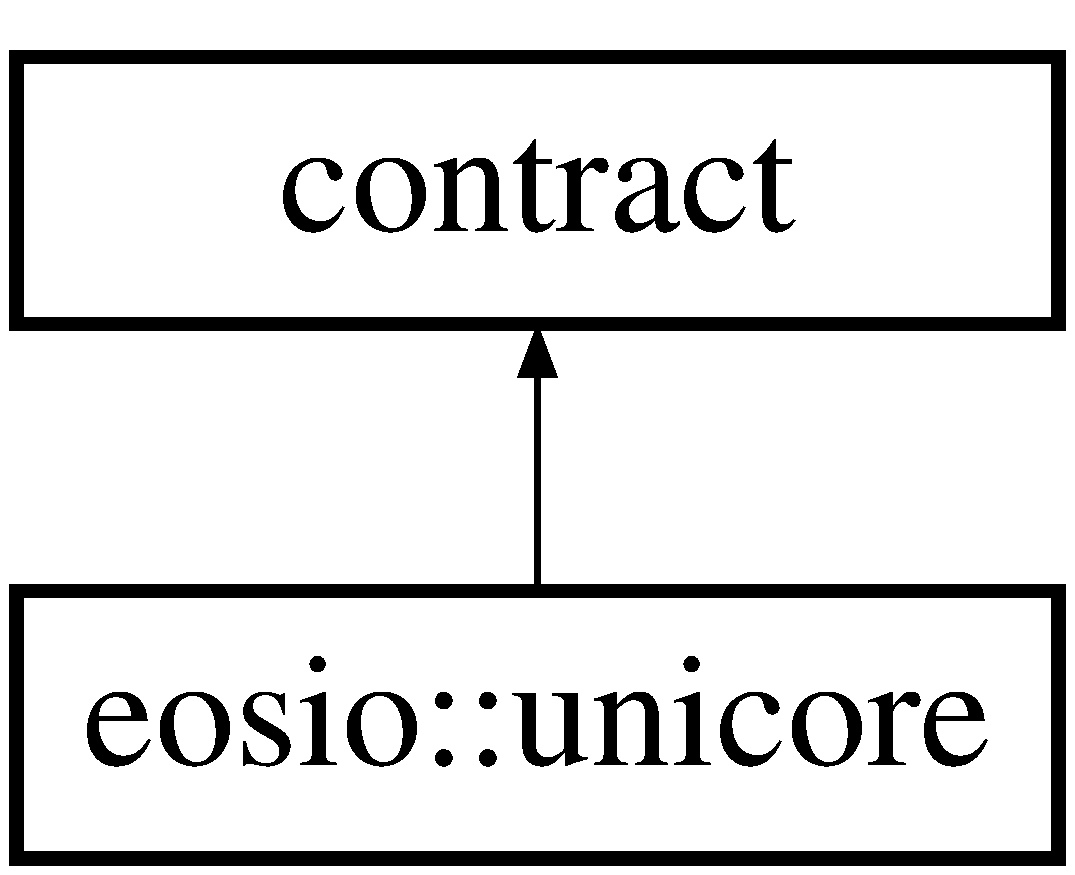
\includegraphics[height=2.000000cm]{classeosio_1_1unicore}
\end{center}
\end{figure}
\subsection*{Public Member Functions}
\begin{DoxyCompactItemize}
\item 
\mbox{\Hypertarget{classeosio_1_1unicore_a6f8aab7d944e62d87dd03562f5ed76a7}\label{classeosio_1_1unicore_a6f8aab7d944e62d87dd03562f5ed76a7}} 
{\bfseries unicore} (eosio\+::name receiver, eosio\+::name code, eosio\+::datastream$<$ const char $\ast$$>$ ds)
\item 
\mbox{\Hypertarget{classeosio_1_1unicore_a59303f0f27f097d80749a7dd0fc084ef}\label{classeosio_1_1unicore_a59303f0f27f097d80749a7dd0fc084ef}} 
void {\bfseries apply} (uint64\+\_\+t receiver, uint64\+\_\+t code, uint64\+\_\+t action)
\item 
\mbox{\Hypertarget{classeosio_1_1unicore_a8a39c3fdbe0d6a386452d1c1f9bd3f27}\label{classeosio_1_1unicore_a8a39c3fdbe0d6a386452d1c1f9bd3f27}} 
void \mbox{\hyperlink{classeosio_1_1unicore_a8a39c3fdbe0d6a386452d1c1f9bd3f27}{convert}} (eosio\+::name username, eosio\+::name host, uint64\+\_\+t balance\+\_\+id)
\begin{DoxyCompactList}\small\item\em Публичный метод обмена баланса на жетон распределения по текущему курсу из числа квантов раунда. \end{DoxyCompactList}\item 
void \mbox{\hyperlink{classeosio_1_1unicore_ac4def2358ff27c9454fcbbb71163f300}{setparams}} (eosio\+::name host, eosio\+::name chost, uint64\+\_\+t size\+\_\+of\+\_\+pool, uint64\+\_\+t quants\+\_\+precision, uint64\+\_\+t overlap, uint64\+\_\+t profit\+\_\+growth, uint64\+\_\+t base\+\_\+rate, uint64\+\_\+t loss\+\_\+percent, uint64\+\_\+t pool\+\_\+limit, uint64\+\_\+t pool\+\_\+timeout, uint64\+\_\+t priority\+\_\+seconds)
\begin{DoxyCompactList}\small\item\em Публичный метод установки параметров протокола двойной спирали Вызывается пользователем после базовой операции создания хоста и проведения оплаты. Так же вызывается при установке параметров дочернего хоста. Содержит алгоритм финансового ядра. Производит основные расчеты таблиц курсов и валидирует положительность бизнес-\/дохода. \end{DoxyCompactList}\item 
void \mbox{\hyperlink{classeosio_1_1unicore_a6d49834320bcf0133e9399a3b45ac3e5}{start}} (eosio\+::name host, eosio\+::name chost)
\begin{DoxyCompactList}\small\item\em Публичный метод запуска хоста Метод необходимо вызвать для запуска хоста после установки параметров хоста. Добавляет первый цикл, два пула, переключает демонастративный флаг запуска и создает статистические объекты. Подписывается аккаунтом хоста. \end{DoxyCompactList}\item 
void \mbox{\hyperlink{classeosio_1_1unicore_a8ffe452ddc02c7f74b0c5e00f0aa22a7}{withdraw}} (eosio\+::name username, eosio\+::name host, uint64\+\_\+t balance\+\_\+id)
\begin{DoxyCompactList}\small\item\em Публичный метод возврата баланса протоколу. Вывод средств возможен только для полностью обновленных (актуальных) балансов. Производит обмен Юнитов на управляющий токен и выплачивает на аккаунт пользователя. \end{DoxyCompactList}\item 
void \mbox{\hyperlink{classeosio_1_1unicore_a8480c8a1d1a04720e7935f8e711d2237}{priorenter}} (eosio\+::name username, eosio\+::name host, uint64\+\_\+t balance\+\_\+id)
\begin{DoxyCompactList}\small\item\em Метод приоритетного входа в новый цикл. Доступен к использованию только при условии наличия предыдущего цикла, в котором участник имеет проигравший баланс. Позволяет зайти частью своего проигравшего баланса одновременно в два пула -\/ первый и второй нового цикла. Использование приоритетного входа возможно только до истечения времени приоритета, которое начинается в момент запуска цикла и продолжается до истечения таймера приоритета. \end{DoxyCompactList}\item 
void \mbox{\hyperlink{classeosio_1_1unicore_ae700163ca48edef7b391531e3dd220c2}{refreshbal}} (eosio\+::name username, uint64\+\_\+t balance\+\_\+id, uint64\+\_\+t partrefresh)
\begin{DoxyCompactList}\small\item\em Публичный метод обновления баланса Пересчет баланса каждого пользователя происходит по его собственному действию. Обновление баланса приводит к пересчету доступной суммы для вывода. \end{DoxyCompactList}\item 
\mbox{\Hypertarget{classeosio_1_1unicore_a72fbcf27ed2d36be0075117b00599482}\label{classeosio_1_1unicore_a72fbcf27ed2d36be0075117b00599482}} 
void {\bfseries init} (uint64\+\_\+t system\+\_\+income)
\item 
void \mbox{\hyperlink{classeosio_1_1unicore_a9ba153178009033b25fdd4db4c36e02e}{refreshst}} (eosio\+::name host)
\begin{DoxyCompactList}\small\item\em Публичный метод обновления состояния Проверяет пул на истечение во времени или завершение целого количества ядерных Юнитов. Запускает новый цикл или добавляет новый пул. \end{DoxyCompactList}\item 
\mbox{\Hypertarget{classeosio_1_1unicore_a46cd90e0a4f1b938d4548ca254782cfe}\label{classeosio_1_1unicore_a46cd90e0a4f1b938d4548ca254782cfe}} 
void {\bfseries setbadge} (uint64\+\_\+t id, eosio\+::name host, eosio\+::string caption, eosio\+::string description, eosio\+::string iurl, eosio\+::string pic, uint64\+\_\+t total, uint64\+\_\+t \mbox{\hyperlink{structpower}{power}})
\item 
\mbox{\Hypertarget{classeosio_1_1unicore_a40fa6e2fa9fcddf76ba73b261eae6fef}\label{classeosio_1_1unicore_a40fa6e2fa9fcddf76ba73b261eae6fef}} 
void {\bfseries giftbadge} (eosio\+::name host, eosio\+::name to, uint64\+\_\+t badge\+\_\+id, eosio\+::string comment, bool netted, uint64\+\_\+t goal\+\_\+id, uint64\+\_\+t task\+\_\+id)
\item 
void \mbox{\hyperlink{classeosio_1_1unicore_a6e7db779eb5836300fabe105012388c2}{backbadge}} (eosio\+::name host, eosio\+::name from, uint64\+\_\+t usbadge\+\_\+id, eosio\+::string comment)
\begin{DoxyCompactList}\small\item\em Метод возврата значка Может быть использован хостом для возврата выданного значка. \end{DoxyCompactList}\item 
void \mbox{\hyperlink{classeosio_1_1unicore_abab6ddd4a167efde5f0e45a1ffd9dfba}{setcontent}} (eosio\+::name username, eosio\+::name type, eosio\+::name lang, eosio\+::string content)
\begin{DoxyCompactList}\small\item\em Модуль C\+MS Позволяет каждому сообществу использовать веб-\/конструктор приложений U\+NI. \end{DoxyCompactList}\item 
void \mbox{\hyperlink{classeosio_1_1unicore_af6aac321d5880fcb577ba00abea5c38f}{rmcontent}} (eosio\+::name username, eosio\+::name type)
\begin{DoxyCompactList}\small\item\em Метод удаления языкового файла \end{DoxyCompactList}\item 
void \mbox{\hyperlink{classeosio_1_1unicore_ad0188feae42e22b52afbb6e3c3f70c86}{setcmsconfig}} (eosio\+::name username, eosio\+::string config)
\begin{DoxyCompactList}\small\item\em Метод установки C\+M\+S-\/конфига \end{DoxyCompactList}\item 
void \mbox{\hyperlink{classeosio_1_1unicore_aa2341c3f2393be329d759ef09f20367f}{setgoal}} (eosio\+::name creator, eosio\+::name host, eosio\+::name type, std\+::string title, std\+::string permlink, std\+::string description, eosio\+::asset target, uint64\+\_\+t duration, uint64\+\_\+t cashback, bool activated, bool is\+\_\+batch, uint64\+\_\+t parent\+\_\+batch\+\_\+id, std\+::string meta)
\begin{DoxyCompactList}\small\item\em Метод создания цели \end{DoxyCompactList}\item 
void \mbox{\hyperlink{classeosio_1_1unicore_a969e75dd90699b53b75ab8482cbc49d3}{dfundgoal}} (eosio\+::name architect, eosio\+::name host, uint64\+\_\+t goal\+\_\+id, eosio\+::asset amount, std\+::string comment)
\begin{DoxyCompactList}\small\item\em Метод прямого финансирования цели Используется архитектором для финансирования цели из фонда \end{DoxyCompactList}\item 
void \mbox{\hyperlink{classeosio_1_1unicore_a9fd534e0b189439c6f18e99689911b3e}{delgoal}} (eosio\+::name username, eosio\+::name host, uint64\+\_\+t goal\+\_\+id)
\begin{DoxyCompactList}\small\item\em Метод удаления цели \end{DoxyCompactList}\item 
void \mbox{\hyperlink{classeosio_1_1unicore_ac0e6bf94b8bfd28e08c364631a357d91}{report}} (eosio\+::name username, eosio\+::name host, uint64\+\_\+t goal\+\_\+id, std\+::string report)
\begin{DoxyCompactList}\small\item\em Метод создания отчета о завершенной цели \end{DoxyCompactList}\item 
void \mbox{\hyperlink{classeosio_1_1unicore_ac31cf68445b14c4dbdea9684a0556f10}{check}} (eosio\+::name architect, eosio\+::name host, uint64\+\_\+t goal\+\_\+id)
\begin{DoxyCompactList}\small\item\em Метод проверки отчета Отчет о достижении цели на текущий момент проверяется только архитектором. \end{DoxyCompactList}\item 
void \mbox{\hyperlink{classeosio_1_1unicore_a4faa41a68505840e66f78e350412723c}{gwithdraw}} (eosio\+::name username, eosio\+::name host, uint64\+\_\+t goal\+\_\+id)
\begin{DoxyCompactList}\small\item\em Метод вывода баланса цели Выводит доступный баланс цели на аккаунт создателя цели. \end{DoxyCompactList}\item 
void \mbox{\hyperlink{classeosio_1_1unicore_a621817942c7b2758963d4147170b3c60}{gsponsor}} (eosio\+::name hoperator, eosio\+::name host, eosio\+::name reciever, uint64\+\_\+t goal\+\_\+id, eosio\+::asset amount)
\begin{DoxyCompactList}\small\item\em Метод финансирования цели через оператора сообщества. Позволяет оператору сообщества расходовать баланс целей на перечисления прямым спонсорам. Используется в риверсной экономической модели, когда корневой токен сообщества является котировочным токеном силы сообщества, и накаким другим способом изначально не распределяется, кроме как на спонсоров целей (дефицитная I\+CO -\/ модель). \end{DoxyCompactList}\item 
void \mbox{\hyperlink{classeosio_1_1unicore_affa39993f35c8e2c8838a956c761cbcc}{setemi}} (eosio\+::name host, uint64\+\_\+t percent, uint64\+\_\+t gtop)
\begin{DoxyCompactList}\small\item\em Метод установки скорости эмиссии и размера листа финансирования \end{DoxyCompactList}\item 
\mbox{\Hypertarget{classeosio_1_1unicore_a1dc8fafea638915880cc4cc44936c3ca}\label{classeosio_1_1unicore_a1dc8fafea638915880cc4cc44936c3ca}} 
void \mbox{\hyperlink{classeosio_1_1unicore_a1dc8fafea638915880cc4cc44936c3ca}{enablesale}} (eosio\+::name host, eosio\+::name token\+\_\+contract, eosio\+::asset asset\+\_\+on\+\_\+sale, int64\+\_\+t sale\+\_\+shift, eosio\+::name sale\+\_\+mode)
\begin{DoxyCompactList}\small\item\em Публичный метод включения сейла с хоста. Может быть использован только до вызова метода start при условии, что владелец контракта токена разрешил это. Активирует реализацию управляющего жетона из фонда владельца жетона в режиме финансового котла. \end{DoxyCompactList}\item 
\mbox{\Hypertarget{classeosio_1_1unicore_a037002fae9b03f0be026da9ae93a46cc}\label{classeosio_1_1unicore_a037002fae9b03f0be026da9ae93a46cc}} 
void \mbox{\hyperlink{classeosio_1_1unicore_a037002fae9b03f0be026da9ae93a46cc}{addhostofund}} (uint64\+\_\+t fund\+\_\+id, eosio\+::name host)
\begin{DoxyCompactList}\small\item\em Публичный метод подключения хоста к фонду \end{DoxyCompactList}\item 
\mbox{\Hypertarget{classeosio_1_1unicore_aa5475ba948281a1c03d8d71277a0edc5}\label{classeosio_1_1unicore_aa5475ba948281a1c03d8d71277a0edc5}} 
void {\bfseries rmhosfrfund} (uint64\+\_\+t fund\+\_\+id, eosio\+::name host)
\item 
\mbox{\Hypertarget{classeosio_1_1unicore_a216b978479f2525fd8d163731a26e60b}\label{classeosio_1_1unicore_a216b978479f2525fd8d163731a26e60b}} 
void \mbox{\hyperlink{classeosio_1_1unicore_a216b978479f2525fd8d163731a26e60b}{transfromgf}} (eosio\+::name to, eosio\+::name token\+\_\+contract, eosio\+::asset quantity)
\begin{DoxyCompactList}\small\item\em Публичный метод перевода из глобального фонда \end{DoxyCompactList}\item 
void \mbox{\hyperlink{classeosio_1_1unicore_a60fc5c05f0fcb57d28def1edd88bc609}{setarch}} (eosio\+::name host, eosio\+::name architect)
\begin{DoxyCompactList}\small\item\em Sets the architect. Устанавливает архитектора сообщества, обладающего полномочиями специальных действий. \end{DoxyCompactList}\item 
void \mbox{\hyperlink{classeosio_1_1unicore_a4924fb028294b806d137c7d1934868f2}{upgrade}} (eosio\+::name username, eosio\+::name platform, std\+::string title, std\+::string purpose, uint64\+\_\+t total\+\_\+shares, eosio\+::asset quote\+\_\+amount, eosio\+::name quote\+\_\+token\+\_\+contract, eosio\+::asset root\+\_\+token, eosio\+::name root\+\_\+token\+\_\+contract, bool voting\+\_\+only\+\_\+up, uint64\+\_\+t consensus\+\_\+percent, uint64\+\_\+t referral\+\_\+percent, uint64\+\_\+t dacs\+\_\+percent, uint64\+\_\+t cfund\+\_\+percent, uint64\+\_\+t hfund\+\_\+percent, std\+::vector$<$ uint64\+\_\+t $>$ levels, uint64\+\_\+t emission\+\_\+percent, uint64\+\_\+t gtop, std\+::string meta)
\begin{DoxyCompactList}\small\item\em Метод апгрейда аккаунта до статуса сообщества Принимает ряд параметров, такие как процент консенсуса, реферальный процент, уровни вознаграждений финансовых партнеров, корпоративный процент, а так же параметры рынка силы. \end{DoxyCompactList}\item 
void \mbox{\hyperlink{classeosio_1_1unicore_a2e3b22660c9e7743bc8659eb0095a81d}{cchildhost}} (eosio\+::name parent\+\_\+host, eosio\+::name chost)
\begin{DoxyCompactList}\small\item\em Метод создания дочернего хоста Позволяет сообществу на границе циклов изменять параметры финансового ядра, распологая их в области памяти аккаунта дочернего хоста. \end{DoxyCompactList}\item 
void \mbox{\hyperlink{classeosio_1_1unicore_ad60e3d78ee78e8b83d4ac7f179d9fcf9}{edithost}} (eosio\+::name architect, eosio\+::name host, eosio\+::string title, eosio\+::string purpose, eosio\+::string manifest, eosio\+::string meta)
\begin{DoxyCompactList}\small\item\em Метод редактирования информации о хосте \end{DoxyCompactList}\item 
\mbox{\Hypertarget{classeosio_1_1unicore_aec940f4ee8ac54df1de176982048455f}\label{classeosio_1_1unicore_aec940f4ee8ac54df1de176982048455f}} 
void {\bfseries fixs} (eosio\+::name host, uint64\+\_\+t pool\+\_\+num)
\item 
\mbox{\Hypertarget{classeosio_1_1unicore_a14965174d2ecda13a31202add151df41}\label{classeosio_1_1unicore_a14965174d2ecda13a31202add151df41}} 
void {\bfseries settype} (eosio\+::name host, eosio\+::name type)
\item 
void \mbox{\hyperlink{classeosio_1_1unicore_a1883144d494a858ab38e04b9a334d07e}{settiming}} (eosio\+::name host, uint64\+\_\+t pool\+\_\+timeout, uint64\+\_\+t priority\+\_\+seconds)
\begin{DoxyCompactList}\small\item\em Метод редактирования времени \end{DoxyCompactList}\item 
\mbox{\Hypertarget{classeosio_1_1unicore_a81816c4d812ba83b1aab66494f574e90}\label{classeosio_1_1unicore_a81816c4d812ba83b1aab66494f574e90}} 
void {\bfseries setflows} (eosio\+::name host, uint64\+\_\+t ref\+\_\+percent, uint64\+\_\+t dacs\+\_\+percent, uint64\+\_\+t cfund\+\_\+percent, uint64\+\_\+t hfund\+\_\+percent)
\item 
\mbox{\Hypertarget{classeosio_1_1unicore_a1713b099515838ad2e42391f4dd03b6f}\label{classeosio_1_1unicore_a1713b099515838ad2e42391f4dd03b6f}} 
void {\bfseries rmben} (eosio\+::name creator, eosio\+::name username, eosio\+::name host, uint64\+\_\+t goal\+\_\+id)
\item 
\mbox{\Hypertarget{classeosio_1_1unicore_a4c8df6c80a48d2a6f8a73469a470ec2f}\label{classeosio_1_1unicore_a4c8df6c80a48d2a6f8a73469a470ec2f}} 
void {\bfseries addben} (eosio\+::name creator, eosio\+::name username, eosio\+::name host, uint64\+\_\+t goal\+\_\+id, uint64\+\_\+t weight)
\item 
\mbox{\Hypertarget{classeosio_1_1unicore_a0a2ae5cf5fb3cdf3ba23f0948dd5c391}\label{classeosio_1_1unicore_a0a2ae5cf5fb3cdf3ba23f0948dd5c391}} 
void {\bfseries withdrbeninc} (eosio\+::name username, eosio\+::name host, uint64\+\_\+t goal\+\_\+id)
\item 
\mbox{\Hypertarget{classeosio_1_1unicore_a47013cbd65e12ca4108ea5fa682570ac}\label{classeosio_1_1unicore_a47013cbd65e12ca4108ea5fa682570ac}} 
void {\bfseries adddac} (eosio\+::name username, eosio\+::name host, uint64\+\_\+t weight, bool is\+\_\+new\+\_\+role, uint64\+\_\+t role\+\_\+id, std\+::string title, std\+::string descriptor)
\item 
\mbox{\Hypertarget{classeosio_1_1unicore_ae659916fb37ee05a3e0ddfeadf63b8eb}\label{classeosio_1_1unicore_ae659916fb37ee05a3e0ddfeadf63b8eb}} 
void {\bfseries rmdac} (eosio\+::name username, eosio\+::name host)
\item 
\mbox{\Hypertarget{classeosio_1_1unicore_ae3a39d90bc3bcf2b02696486b5e8026c}\label{classeosio_1_1unicore_ae3a39d90bc3bcf2b02696486b5e8026c}} 
void {\bfseries suggestrole} (eosio\+::name username, std\+::string title, std\+::string descriptor)
\item 
\mbox{\Hypertarget{classeosio_1_1unicore_a6969c7a238ad81c459428566276c6606}\label{classeosio_1_1unicore_a6969c7a238ad81c459428566276c6606}} 
void {\bfseries withdrdacinc} (eosio\+::name username, eosio\+::name host)
\item 
\mbox{\Hypertarget{classeosio_1_1unicore_a40f34fee3046e08d4ff00aa1fa94acab}\label{classeosio_1_1unicore_a40f34fee3046e08d4ff00aa1fa94acab}} 
void {\bfseries setwebsite} (eosio\+::name host, eosio\+::name ahostname, eosio\+::string website, eosio\+::name type)
\item 
\mbox{\Hypertarget{classeosio_1_1unicore_aa678c5b5e9eba7ae59090ab05e6fbb79}\label{classeosio_1_1unicore_aa678c5b5e9eba7ae59090ab05e6fbb79}} 
void {\bfseries rmahost} (eosio\+::name host, eosio\+::name ahostname)
\item 
\mbox{\Hypertarget{classeosio_1_1unicore_ac716bdbd92457fa5f79abe23c5c3cd60}\label{classeosio_1_1unicore_ac716bdbd92457fa5f79abe23c5c3cd60}} 
void {\bfseries setahost} (eosio\+::name host, eosio\+::name ahostname)
\item 
\mbox{\Hypertarget{classeosio_1_1unicore_a62874f2d37da9ba4732e184c8a78cbdc}\label{classeosio_1_1unicore_a62874f2d37da9ba4732e184c8a78cbdc}} 
void {\bfseries closeahost} (eosio\+::name host)
\item 
\mbox{\Hypertarget{classeosio_1_1unicore_a593ba94cb5031d9dd492f10a3fa8189c}\label{classeosio_1_1unicore_a593ba94cb5031d9dd492f10a3fa8189c}} 
void {\bfseries openahost} (eosio\+::name host)
\item 
void \mbox{\hyperlink{classeosio_1_1unicore_acd107f6210ac17a454adf216765151f2}{refreshsh}} (eosio\+::name owner, uint64\+\_\+t id)
\begin{DoxyCompactList}\small\item\em Метод обновления вестинг-\/баланса. ~\newline
Обновляет вестинг-\/баланс до актуальных параметров продолжительности. \end{DoxyCompactList}\item 
\mbox{\Hypertarget{classeosio_1_1unicore_a46d07ca7ccd7d5d04c6357c0c2d36209}\label{classeosio_1_1unicore_a46d07ca7ccd7d5d04c6357c0c2d36209}} 
void \mbox{\hyperlink{classeosio_1_1unicore_a46d07ca7ccd7d5d04c6357c0c2d36209}{withpbenefit}} (eosio\+::name username, eosio\+::name host)
\begin{DoxyCompactList}\small\item\em Метод вывода силового финансового потока withdraw power quant (withpowerun) Позволяет вывести часть финансового потока, направленного на держателя силы \end{DoxyCompactList}\item 
\mbox{\Hypertarget{classeosio_1_1unicore_a61e8b58df156894fdb10e7609e6dd7ef}\label{classeosio_1_1unicore_a61e8b58df156894fdb10e7609e6dd7ef}} 
void \mbox{\hyperlink{classeosio_1_1unicore_a61e8b58df156894fdb10e7609e6dd7ef}{withrsegment}} (eosio\+::name username, eosio\+::name host)
\begin{DoxyCompactList}\small\item\em Метод вывода остатка партнерского финансового потока withdraw power quant (withpowerun) \end{DoxyCompactList}\item 
\mbox{\Hypertarget{classeosio_1_1unicore_aeb9e4fcea08c5e5c198c89e1390ac80e}\label{classeosio_1_1unicore_aeb9e4fcea08c5e5c198c89e1390ac80e}} 
void \mbox{\hyperlink{classeosio_1_1unicore_aeb9e4fcea08c5e5c198c89e1390ac80e}{withrbenefit}} (eosio\+::name username, eosio\+::name host, std\+::vector$<$ uint64\+\_\+t $>$ ids)
\begin{DoxyCompactList}\small\item\em Метод вывода партнерского финансового потока withdraw power quant (withpowerun) \end{DoxyCompactList}\item 
void \mbox{\hyperlink{classeosio_1_1unicore_adc22e2d70fc4e3cb6a72b26a1d82186a}{refreshpu}} (eosio\+::name username, eosio\+::name host)
\begin{DoxyCompactList}\small\item\em Метод обновления силового финансового потока \end{DoxyCompactList}\item 
void \mbox{\hyperlink{classeosio_1_1unicore_a46b78c56992d90f8e41f05c62f7900cd}{withdrawsh}} (eosio\+::name owner, uint64\+\_\+t id)
\begin{DoxyCompactList}\small\item\em Вывод вестинг-\/баланса Обеспечивает вывод доступных средств из вестинг-\/баланса. \end{DoxyCompactList}\item 
void \mbox{\hyperlink{classeosio_1_1unicore_a40ab650798ac7b7ce35f42526a217e44}{sellshares}} (eosio\+::name username, eosio\+::name host, uint64\+\_\+t shares)
\begin{DoxyCompactList}\small\item\em Публичный метод продажи силы рынку за котировочный токен \end{DoxyCompactList}\item 
void \mbox{\hyperlink{classeosio_1_1unicore_a20ec8fa3451334f2920a0b9b501dae6c}{undelshares}} (eosio\+::name from, eosio\+::name reciever, eosio\+::name host, uint64\+\_\+t shares)
\begin{DoxyCompactList}\small\item\em Метод возврата делегированной силы \end{DoxyCompactList}\item 
void \mbox{\hyperlink{classeosio_1_1unicore_acfa60cf59df336c954662c1ae46a67b2}{settask}} (eosio\+::name host, eosio\+::name creator, std\+::string permlink, uint64\+\_\+t goal\+\_\+id, uint64\+\_\+t priority, eosio\+::string title, eosio\+::string data, eosio\+::asset requested, bool is\+\_\+public, eosio\+::name doer, eosio\+::asset for\+\_\+each, bool with\+\_\+badge, uint64\+\_\+t badge\+\_\+id, uint64\+\_\+t duration, bool is\+\_\+batch, uint64\+\_\+t parent\+\_\+batch\+\_\+id, std\+::string meta)
\begin{DoxyCompactList}\small\item\em Модуль задач Задачи есть составляющие части достижения любой цели. Постановка задач осуществляется только в рамках целей. Задачи могут быть \end{DoxyCompactList}\item 
void \mbox{\hyperlink{classeosio_1_1unicore_ae8ca388e55f11d3c32430edbaabcf7e2}{fundtask}} (eosio\+::name host, uint64\+\_\+t task\+\_\+id, eosio\+::asset amount, eosio\+::string comment)
\begin{DoxyCompactList}\small\item\em Публичный метод фондирования задачи Исполняется хостом для пополнения баланса задачи из доступного баланса цели. \end{DoxyCompactList}\item 
void \mbox{\hyperlink{classeosio_1_1unicore_a0c35d9830c0c05c8f13be48b8cbdf236}{tactivate}} (eosio\+::name host, uint64\+\_\+t task\+\_\+id)
\begin{DoxyCompactList}\small\item\em Метод активации задачи Вызывается хостом для активации выполнения поставленной задачи. \end{DoxyCompactList}\item 
void \mbox{\hyperlink{classeosio_1_1unicore_a725477908310816ec80cddbf733af04b}{tdeactivate}} (eosio\+::name host, uint64\+\_\+t task\+\_\+id)
\begin{DoxyCompactList}\small\item\em Публичный метод деактивации задачи Применимо для публичных задач, когда поставленная цель достигнута или недостижима. \end{DoxyCompactList}\item 
void \mbox{\hyperlink{classeosio_1_1unicore_a09d7d2d602069a26875aa1eee250d5f4}{deltask}} (eosio\+::name host, uint64\+\_\+t task\+\_\+id)
\begin{DoxyCompactList}\small\item\em Метод удаления задачи Вызывается хостом для удаления поставленной задачи. \end{DoxyCompactList}\item 
void \mbox{\hyperlink{classeosio_1_1unicore_ab10a203c3d6c37fd1cb71a9110c62e8a}{paydebt}} (eosio\+::name host, uint64\+\_\+t goal\+\_\+id)
\begin{DoxyCompactList}\small\item\em Метод выплаты долга по цели из числа available в счет объектов долга \end{DoxyCompactList}\item 
void \mbox{\hyperlink{classeosio_1_1unicore_a178fc39ee1d642454bddeaa3f6084d00}{setreport}} (eosio\+::name host, eosio\+::name username, uint64\+\_\+t task\+\_\+id, eosio\+::string data)
\begin{DoxyCompactList}\small\item\em Публичный метод создания отчета о выполненной задаче Применяется исполнителем задачи для того, чтобы отправить отчет на проверку. \end{DoxyCompactList}\item 
void \mbox{\hyperlink{classeosio_1_1unicore_ad041a75ade13b77f67f54c99f7ca7d29}{editreport}} (eosio\+::name host, eosio\+::name username, uint64\+\_\+t report\+\_\+id, eosio\+::string data)
\begin{DoxyCompactList}\small\item\em Публиный метод редактирования отчета В случае, если отчет не принят, участник получает возможность отредактировать свой отчет и выслать его на проверку повторно. \end{DoxyCompactList}\item 
void \mbox{\hyperlink{classeosio_1_1unicore_a765b3c6b36dc26922fec8c1236e3d154}{approver}} (eosio\+::name host, uint64\+\_\+t report\+\_\+id, eosio\+::string comment)
\begin{DoxyCompactList}\small\item\em Публичный метод одобрения отчета Используется хостом для того, чтобы принять задачу как выполненную и выдать вознаграждение / награду в виде значка. \end{DoxyCompactList}\item 
void \mbox{\hyperlink{classeosio_1_1unicore_a403175c6abbcf360d36ec0259bccc109}{disapprover}} (eosio\+::name host, uint64\+\_\+t report\+\_\+id, eosio\+::string comment)
\begin{DoxyCompactList}\small\item\em Публичный метод отклонения отчета \end{DoxyCompactList}\item 
\mbox{\Hypertarget{classeosio_1_1unicore_a9f959b326fccc37b6d0edff7ac941c77}\label{classeosio_1_1unicore_a9f959b326fccc37b6d0edff7ac941c77}} 
void {\bfseries vote} (eosio\+::name voter, eosio\+::name host, uint64\+\_\+t goal\+\_\+id, bool up)
\item 
\mbox{\Hypertarget{classeosio_1_1unicore_a11379b173a7701fce57491ed285a7f24}\label{classeosio_1_1unicore_a11379b173a7701fce57491ed285a7f24}} 
void {\bfseries setcondition} (eosio\+::name host, eosio\+::string key, uint64\+\_\+t value)
\item 
\mbox{\Hypertarget{classeosio_1_1unicore_a600c89c52dedf76705f46bc2caef60f7}\label{classeosio_1_1unicore_a600c89c52dedf76705f46bc2caef60f7}} 
void {\bfseries rmcondition} (eosio\+::name host, uint64\+\_\+t key)
\item 
std\+::string \mbox{\hyperlink{classeosio_1_1unicore_a2464971a6336dedb991282d0b396177e}{symbol\+\_\+to\+\_\+string}} (eosio\+::asset val) const
\begin{DoxyCompactList}\small\item\em Структура хоста \end{DoxyCompactList}\end{DoxyCompactItemize}
\subsection*{Static Public Member Functions}
\begin{DoxyCompactItemize}
\item 
\mbox{\Hypertarget{classeosio_1_1unicore_a636683722a5dfb0a416b26888a78186c}\label{classeosio_1_1unicore_a636683722a5dfb0a416b26888a78186c}} 
static eosio\+::asset {\bfseries convert\+\_\+to\+\_\+power} (eosio\+::asset quantity, eosio\+::name host)
\item 
static void \mbox{\hyperlink{classeosio_1_1unicore_af4376715edeb68b09c6921cd4d101345}{pay\+\_\+for\+\_\+upgrade}} (eosio\+::name username, eosio\+::asset amount, eosio\+::name code)
\begin{DoxyCompactList}\small\item\em Метод оплаты комиссии создания дочернего хоста \end{DoxyCompactList}\item 
\mbox{\Hypertarget{classeosio_1_1unicore_af67dcbc765acec01896202ca20159ecf}\label{classeosio_1_1unicore_af67dcbc765acec01896202ca20159ecf}} 
static void {\bfseries refresh\+\_\+state} (eosio\+::name host)
\item 
static void \mbox{\hyperlink{classeosio_1_1unicore_a5e0d285466d37fa9f315b5a52dba4c8a}{giftbadge\+\_\+action}} (eosio\+::name host, eosio\+::name to, uint64\+\_\+t badge\+\_\+id, eosio\+::string comment, bool netted, uint64\+\_\+t goal\+\_\+id, uint64\+\_\+t task\+\_\+id)
\begin{DoxyCompactList}\small\item\em Метод передачи значка награждаемому \end{DoxyCompactList}\item 
\mbox{\Hypertarget{classeosio_1_1unicore_a77606350bcf0ef3b500a0cf29b754311}\label{classeosio_1_1unicore_a77606350bcf0ef3b500a0cf29b754311}} 
static void {\bfseries deposit} (eosio\+::name username, eosio\+::name host, eosio\+::asset amount, eosio\+::name code, std\+::string message)
\item 
static void \mbox{\hyperlink{classeosio_1_1unicore_a466aba74657c6022cc0d9163bd502625}{donate\+\_\+action}} (eosio\+::name from, eosio\+::name host, uint64\+\_\+t goal\+\_\+id, eosio\+::asset quantity, eosio\+::name code)
\begin{DoxyCompactList}\small\item\em Метод спонсорского взноса на цель Позволяет любому участнику произвести финансирование цели из числа собственных средств. \end{DoxyCompactList}\item 
static eosio\+::asset \mbox{\hyperlink{classeosio_1_1unicore_acd0fd09c0cbd6459684222639c98d628}{adjust\+\_\+goals\+\_\+emission\+\_\+pool}} (eosio\+::name hostname)
\begin{DoxyCompactList}\small\item\em Внутренний метод расчета пула эмиссии. Вызывается в момент распределения эмиссии на цели сообщества. Расчет объема эмиссии происходит исходя из параметра life\+\_\+balance\+\_\+for\+\_\+sale завершенного пула, и процента эмиссии, установленного архитектором. Процент эмиссии ограничен от 0 до 1000\% относительного живого остатка на продажу в каждом новом пуле. \end{DoxyCompactList}\item 
static void \mbox{\hyperlink{classeosio_1_1unicore_a728e6dc69d5a0ce303b504b299bfdb4b}{fund\+\_\+emi\+\_\+pool}} (eosio\+::name host, eosio\+::asset amount, eosio\+::name code)
\begin{DoxyCompactList}\small\item\em Метод ручного пополнения целевого фонда сообщества. Жетоны, попадающие в целевой фонд сообщества, подлежат распределению на цели с помощью голосования участников по установленным правилам консенсуса. \end{DoxyCompactList}\item 
\mbox{\Hypertarget{classeosio_1_1unicore_a136440444a225070ea36fe6497643c99}\label{classeosio_1_1unicore_a136440444a225070ea36fe6497643c99}} 
static void \mbox{\hyperlink{classeosio_1_1unicore_a136440444a225070ea36fe6497643c99}{add\+\_\+asset\+\_\+to\+\_\+fund\+\_\+action}} (eosio\+::name username, eosio\+::asset quantity, eosio\+::name code)
\begin{DoxyCompactList}\small\item\em Публичный метод пополнения фонда \end{DoxyCompactList}\item 
\mbox{\Hypertarget{classeosio_1_1unicore_a238e2f31fcf0852534c411eacecfeb3c}\label{classeosio_1_1unicore_a238e2f31fcf0852534c411eacecfeb3c}} 
static void \mbox{\hyperlink{classeosio_1_1unicore_a238e2f31fcf0852534c411eacecfeb3c}{createfund}} (eosio\+::name token\+\_\+contract, eosio\+::asset fund\+\_\+asset, std\+::string descriptor)
\begin{DoxyCompactList}\small\item\em Статичный метод создания фонда \end{DoxyCompactList}\item 
\mbox{\Hypertarget{classeosio_1_1unicore_adfeb4fb3878a10d4acf6dc472566bc55}\label{classeosio_1_1unicore_adfeb4fb3878a10d4acf6dc472566bc55}} 
static eosio\+::asset \mbox{\hyperlink{classeosio_1_1unicore_adfeb4fb3878a10d4acf6dc472566bc55}{buy\+\_\+action}} (eosio\+::name username, eosio\+::name host, eosio\+::asset quantity, eosio\+::name code, bool transfer, bool spread\+\_\+to\+\_\+funds, eosio\+::asset summ)
\begin{DoxyCompactList}\small\item\em Публичный метод покупки по текущему курсу из числа квантов раунда. \end{DoxyCompactList}\item 
\mbox{\Hypertarget{classeosio_1_1unicore_a5d8ddfb04f14e1b90bc207d20f16e2ae}\label{classeosio_1_1unicore_a5d8ddfb04f14e1b90bc207d20f16e2ae}} 
static void {\bfseries settype\+\_\+static} (eosio\+::name host, eosio\+::name type)
\item 
\mbox{\Hypertarget{classeosio_1_1unicore_a26f7df861487d0d3b018376b9b3fea9d}\label{classeosio_1_1unicore_a26f7df861487d0d3b018376b9b3fea9d}} 
static void {\bfseries spread\+\_\+to\+\_\+benefactors} (eosio\+::name host, eosio\+::asset amount, uint64\+\_\+t goal\+\_\+id)
\item 
\mbox{\Hypertarget{classeosio_1_1unicore_a2982652beebd5b83055f71b303a49acb}\label{classeosio_1_1unicore_a2982652beebd5b83055f71b303a49acb}} 
static void {\bfseries spread\+\_\+to\+\_\+dacs} (eosio\+::name host, eosio\+::asset amount)
\item 
\mbox{\Hypertarget{classeosio_1_1unicore_a34e59d6ad061725584e12a0f11bcd713}\label{classeosio_1_1unicore_a34e59d6ad061725584e12a0f11bcd713}} 
static void {\bfseries spread\+\_\+to\+\_\+funds} (eosio\+::name host, uint64\+\_\+t quants)
\item 
static uint64\+\_\+t \mbox{\hyperlink{classeosio_1_1unicore_a4e744b6a55f783f4f70a9d43a23daf98}{buyshares\+\_\+action}} (eosio\+::name buyer, eosio\+::name host, eosio\+::asset amount, eosio\+::name code)
\begin{DoxyCompactList}\small\item\em Метод покупки силы сообщества Обеспечивает покупку силы сообщества за котировочный токен по внутренней рыночной цене, определяемой с помощью алгоритма банкор. \end{DoxyCompactList}\item 
static void \mbox{\hyperlink{classeosio_1_1unicore_a911405ecb8c408e127196c9b27401f9f}{delegate\+\_\+shares\+\_\+action}} (eosio\+::name from, eosio\+::name reciever, eosio\+::name host, uint64\+\_\+t shares)
\begin{DoxyCompactList}\small\item\em Метод делегирования силы. Позволяет делегировать купленную силу для принятия каких-\/либо решений в пользу любого аккаунта. \end{DoxyCompactList}\item 
static void \mbox{\hyperlink{classeosio_1_1unicore_a109b4a1d03b051e6d42a746d245ece71}{propagate\+\_\+votes\+\_\+changes}} (eosio\+::name host, eosio\+::name voter, uint64\+\_\+t old\+\_\+power, uint64\+\_\+t new\+\_\+power)
\begin{DoxyCompactList}\small\item\em Обновление счетчика голосов Внутренний метод, используемый для обновления голосов у целей в момент покупки/продажи силы. \end{DoxyCompactList}\item 
\mbox{\Hypertarget{classeosio_1_1unicore_a2621edaa340a06b0b3140ed1e665aced}\label{classeosio_1_1unicore_a2621edaa340a06b0b3140ed1e665aced}} 
static void {\bfseries rmfromhostwl} (eosio\+::name host, eosio\+::name username)
\item 
\mbox{\Hypertarget{classeosio_1_1unicore_af839961f3a9b1b4b0a2a72c4da80b29e}\label{classeosio_1_1unicore_af839961f3a9b1b4b0a2a72c4da80b29e}} 
static void {\bfseries addtohostwl} (eosio\+::name host, eosio\+::name username)
\item 
\mbox{\Hypertarget{classeosio_1_1unicore_af38098cad77812962d2f3190af29b222}\label{classeosio_1_1unicore_af38098cad77812962d2f3190af29b222}} 
static bool {\bfseries checkcondition} (eosio\+::name host, eosio\+::string key, uint64\+\_\+t value)
\item 
\mbox{\Hypertarget{classeosio_1_1unicore_a69f4801c22f9f2c828f5bf8d9170faaa}\label{classeosio_1_1unicore_a69f4801c22f9f2c828f5bf8d9170faaa}} 
static void {\bfseries checkminpwr} (eosio\+::name host, eosio\+::name username)
\item 
\mbox{\Hypertarget{classeosio_1_1unicore_adaef461ff857e01e793f9d8900963f2e}\label{classeosio_1_1unicore_adaef461ff857e01e793f9d8900963f2e}} 
static void {\bfseries change\+\_\+bw\+\_\+trade\+\_\+graph} (eosio\+::name host, uint64\+\_\+t pool\+\_\+id, uint64\+\_\+t cycle\+\_\+num, uint64\+\_\+t pool\+\_\+num, uint64\+\_\+t buy\+\_\+rate, uint64\+\_\+t next\+\_\+buy\+\_\+rate, uint64\+\_\+t total\+\_\+quants, uint64\+\_\+t remain\+\_\+quants, std\+::string color)
\item 
\mbox{\Hypertarget{classeosio_1_1unicore_a46aeb03b30648b83f0b653b3bcb877a2}\label{classeosio_1_1unicore_a46aeb03b30648b83f0b653b3bcb877a2}} 
static void \mbox{\hyperlink{classeosio_1_1unicore_a46aeb03b30648b83f0b653b3bcb877a2}{add\+\_\+coredhistory}} (eosio\+::name host, eosio\+::name username, uint64\+\_\+t pool\+\_\+id, eosio\+::asset amount, std\+::string action, std\+::string message)
\begin{DoxyCompactList}\small\item\em Приватный метод обновления истории ядра \end{DoxyCompactList}\item 
static void \mbox{\hyperlink{classeosio_1_1unicore_a742e69fc7bf0443263f4082845a5325f}{create\+\_\+bancor\+\_\+market}} (std\+::string name, uint64\+\_\+t id, eosio\+::name host, uint64\+\_\+t total\+\_\+shares, eosio\+::asset quote\+\_\+amount, eosio\+::name quote\+\_\+token\+\_\+contract, uint64\+\_\+t vesting\+\_\+seconds)
\begin{DoxyCompactList}\small\item\em Приватный метод создания банкор-\/рынка. \end{DoxyCompactList}\item 
static std\+::vector$<$ eosio\+::asset $>$ \mbox{\hyperlink{classeosio_1_1unicore_a4b687f72582684ca991a201209ec46dd}{calculate\+\_\+forecast}} (eosio\+::name username, eosio\+::name host, uint64\+\_\+t quants, uint64\+\_\+t pool\+\_\+num, eosio\+::asset purchase\+\_\+amount, bool calculate\+\_\+first, bool calculate\+\_\+zero)
\begin{DoxyCompactList}\small\item\em Метод расчета прогнозов Внутренний метод расчета прогнозов. Внутренний метод расчета прогнозов выплат для последующих 8х бассейнов на основе будущих курсов. Используются только для демонастрации. \end{DoxyCompactList}\item 
static void \mbox{\hyperlink{classeosio_1_1unicore_a81f044d8edee706d224c4569581df805}{fill\+\_\+pool}} (eosio\+::name username, eosio\+::name host, uint64\+\_\+t quants, eosio\+::asset amount, uint64\+\_\+t filled\+\_\+pool\+\_\+id)
\begin{DoxyCompactList}\small\item\em Внутренний метод заполнения пула. Вызывается в момент совершения депозита пользователем или на приоритетном входе. Создает баланс пользователю и уменьшает количество квантов в пуле. \end{DoxyCompactList}\item 
\mbox{\Hypertarget{classeosio_1_1unicore_af243d3a5cddb5eb97bafc5cc046818c3}\label{classeosio_1_1unicore_af243d3a5cddb5eb97bafc5cc046818c3}} 
static void {\bfseries check\+\_\+and\+\_\+modify\+\_\+sale\+\_\+fund} (eosio\+::asset amount, \mbox{\hyperlink{structhosts}{hosts}} acc)
\item 
static void \mbox{\hyperlink{classeosio_1_1unicore_a2c500017101260f67b0e8ad3a3b6acfc}{give\+\_\+shares\+\_\+with\+\_\+badge\+\_\+action}} (eosio\+::name host, eosio\+::name reciever, uint64\+\_\+t shares)
\begin{DoxyCompactList}\small\item\em Внутренний метод эмиссии силы. Используется при выдаче знака отличия \end{DoxyCompactList}\item 
static void \mbox{\hyperlink{classeosio_1_1unicore_a01a9d82308c52ec8c93653d310751d2b}{back\+\_\+shares\+\_\+with\+\_\+badge\+\_\+action}} (eosio\+::name host, eosio\+::name from, uint64\+\_\+t shares)
\begin{DoxyCompactList}\small\item\em Внутренний метод возврата силы при возврате значка. Используется при возврате знака отличия хосту \end{DoxyCompactList}\item 
\mbox{\Hypertarget{classeosio_1_1unicore_a9121ac21b1820a4936343c03f1d1a6fe}\label{classeosio_1_1unicore_a9121ac21b1820a4936343c03f1d1a6fe}} 
static void {\bfseries add\+\_\+sale\+\_\+history} (\mbox{\hyperlink{structhosts}{hosts}} acc, \mbox{\hyperlink{structrate}{rate}} \mbox{\hyperlink{structrate}{rate}}, \mbox{\hyperlink{structspiral}{spiral}} sp, eosio\+::asset amount)
\end{DoxyCompactItemize}


\subsection{Member Function Documentation}
\mbox{\Hypertarget{classeosio_1_1unicore_acd0fd09c0cbd6459684222639c98d628}\label{classeosio_1_1unicore_acd0fd09c0cbd6459684222639c98d628}} 
\index{eosio\+::unicore@{eosio\+::unicore}!adjust\+\_\+goals\+\_\+emission\+\_\+pool@{adjust\+\_\+goals\+\_\+emission\+\_\+pool}}
\index{adjust\+\_\+goals\+\_\+emission\+\_\+pool@{adjust\+\_\+goals\+\_\+emission\+\_\+pool}!eosio\+::unicore@{eosio\+::unicore}}
\subsubsection{\texorpdfstring{adjust\+\_\+goals\+\_\+emission\+\_\+pool()}{adjust\_goals\_emission\_pool()}}
{\footnotesize\ttfamily eosio\+::asset eosio\+::unicore\+::adjust\+\_\+goals\+\_\+emission\+\_\+pool (\begin{DoxyParamCaption}\item[{eosio\+::name}]{hostname }\end{DoxyParamCaption})\hspace{0.3cm}{\ttfamily [static]}}



Внутренний метод расчета пула эмиссии. Вызывается в момент распределения эмиссии на цели сообщества. Расчет объема эмиссии происходит исходя из параметра life\+\_\+balance\+\_\+for\+\_\+sale завершенного пула, и процента эмиссии, установленного архитектором. Процент эмиссии ограничен от 0 до 1000\% относительного живого остатка на продажу в каждом новом пуле. 


\begin{DoxyParams}[1]{Parameters}
\mbox{\tt in}  & {\em hostname} & The hostname -\/ имя аккаунта хоста\\
\hline
\end{DoxyParams}
\begin{DoxyReturn}{Returns}
\{ description\+\_\+of\+\_\+the\+\_\+return\+\_\+value \} 
\end{DoxyReturn}
\mbox{\Hypertarget{classeosio_1_1unicore_a765b3c6b36dc26922fec8c1236e3d154}\label{classeosio_1_1unicore_a765b3c6b36dc26922fec8c1236e3d154}} 
\index{eosio\+::unicore@{eosio\+::unicore}!approver@{approver}}
\index{approver@{approver}!eosio\+::unicore@{eosio\+::unicore}}
\subsubsection{\texorpdfstring{approver()}{approver()}}
{\footnotesize\ttfamily void unicore\+::approver (\begin{DoxyParamCaption}\item[{eosio\+::name}]{host,  }\item[{uint64\+\_\+t}]{report\+\_\+id,  }\item[{eosio\+::string}]{comment }\end{DoxyParamCaption})}



Публичный метод одобрения отчета Используется хостом для того, чтобы принять задачу как выполненную и выдать вознаграждение / награду в виде значка. 


\begin{DoxyParams}[1]{Parameters}
\mbox{\tt in}  & {\em op} & The operation \\
\hline
\end{DoxyParams}
\mbox{\Hypertarget{classeosio_1_1unicore_a01a9d82308c52ec8c93653d310751d2b}\label{classeosio_1_1unicore_a01a9d82308c52ec8c93653d310751d2b}} 
\index{eosio\+::unicore@{eosio\+::unicore}!back\+\_\+shares\+\_\+with\+\_\+badge\+\_\+action@{back\+\_\+shares\+\_\+with\+\_\+badge\+\_\+action}}
\index{back\+\_\+shares\+\_\+with\+\_\+badge\+\_\+action@{back\+\_\+shares\+\_\+with\+\_\+badge\+\_\+action}!eosio\+::unicore@{eosio\+::unicore}}
\subsubsection{\texorpdfstring{back\+\_\+shares\+\_\+with\+\_\+badge\+\_\+action()}{back\_shares\_with\_badge\_action()}}
{\footnotesize\ttfamily void eosio\+::unicore\+::back\+\_\+shares\+\_\+with\+\_\+badge\+\_\+action (\begin{DoxyParamCaption}\item[{eosio\+::name}]{host,  }\item[{eosio\+::name}]{from,  }\item[{uint64\+\_\+t}]{shares }\end{DoxyParamCaption})\hspace{0.3cm}{\ttfamily [static]}}



Внутренний метод возврата силы при возврате значка. Используется при возврате знака отличия хосту 


\begin{DoxyParams}[1]{Parameters}
\mbox{\tt in}  & {\em op} & The operation \\
\hline
\end{DoxyParams}
\mbox{\Hypertarget{classeosio_1_1unicore_a6e7db779eb5836300fabe105012388c2}\label{classeosio_1_1unicore_a6e7db779eb5836300fabe105012388c2}} 
\index{eosio\+::unicore@{eosio\+::unicore}!backbadge@{backbadge}}
\index{backbadge@{backbadge}!eosio\+::unicore@{eosio\+::unicore}}
\subsubsection{\texorpdfstring{backbadge()}{backbadge()}}
{\footnotesize\ttfamily void unicore\+::backbadge (\begin{DoxyParamCaption}\item[{eosio\+::name}]{host,  }\item[{eosio\+::name}]{from,  }\item[{uint64\+\_\+t}]{usbadge\+\_\+id,  }\item[{eosio\+::string}]{comment }\end{DoxyParamCaption})}



Метод возврата значка Может быть использован хостом для возврата выданного значка. 


\begin{DoxyParams}[1]{Parameters}
\mbox{\tt in}  & {\em op} & The operation \\
\hline
\end{DoxyParams}
\mbox{\Hypertarget{classeosio_1_1unicore_a4e744b6a55f783f4f70a9d43a23daf98}\label{classeosio_1_1unicore_a4e744b6a55f783f4f70a9d43a23daf98}} 
\index{eosio\+::unicore@{eosio\+::unicore}!buyshares\+\_\+action@{buyshares\+\_\+action}}
\index{buyshares\+\_\+action@{buyshares\+\_\+action}!eosio\+::unicore@{eosio\+::unicore}}
\subsubsection{\texorpdfstring{buyshares\+\_\+action()}{buyshares\_action()}}
{\footnotesize\ttfamily uint64\+\_\+t eosio\+::unicore\+::buyshares\+\_\+action (\begin{DoxyParamCaption}\item[{eosio\+::name}]{buyer,  }\item[{eosio\+::name}]{host,  }\item[{eosio\+::asset}]{amount,  }\item[{eosio\+::name}]{code }\end{DoxyParamCaption})\hspace{0.3cm}{\ttfamily [static]}}



Метод покупки силы сообщества Обеспечивает покупку силы сообщества за котировочный токен по внутренней рыночной цене, определяемой с помощью алгоритма банкор. 


\begin{DoxyParams}[1]{Parameters}
\mbox{\tt in}  & {\em buyer} & The buyer \\
\hline
\mbox{\tt in}  & {\em host} & The host \\
\hline
\mbox{\tt in}  & {\em amount} & The amount \\
\hline
\end{DoxyParams}
\mbox{\Hypertarget{classeosio_1_1unicore_a4b687f72582684ca991a201209ec46dd}\label{classeosio_1_1unicore_a4b687f72582684ca991a201209ec46dd}} 
\index{eosio\+::unicore@{eosio\+::unicore}!calculate\+\_\+forecast@{calculate\+\_\+forecast}}
\index{calculate\+\_\+forecast@{calculate\+\_\+forecast}!eosio\+::unicore@{eosio\+::unicore}}
\subsubsection{\texorpdfstring{calculate\+\_\+forecast()}{calculate\_forecast()}}
{\footnotesize\ttfamily std\+::vector$<$ eosio\+::asset $>$ eosio\+::unicore\+::calculate\+\_\+forecast (\begin{DoxyParamCaption}\item[{eosio\+::name}]{username,  }\item[{eosio\+::name}]{host,  }\item[{uint64\+\_\+t}]{quants,  }\item[{uint64\+\_\+t}]{pool\+\_\+num,  }\item[{eosio\+::asset}]{purchase\+\_\+amount,  }\item[{bool}]{calculate\+\_\+first = {\ttfamily true},  }\item[{bool}]{calculate\+\_\+zero = {\ttfamily false} }\end{DoxyParamCaption})\hspace{0.3cm}{\ttfamily [static]}}



Метод расчета прогнозов Внутренний метод расчета прогнозов. Внутренний метод расчета прогнозов выплат для последующих 8х бассейнов на основе будущих курсов. Используются только для демонастрации. 

T\+O\+DO Может дополнительно быть реализован в качестве внешнего метода достоверной проверки прогнозов, который с каждым вызовом производит расчет будущих курсов и расширяет массив с данными по желанию пользователя. Устранить избыток кода.


\begin{DoxyParams}[1]{Parameters}
\mbox{\tt in}  & {\em username} & The username \\
\hline
\mbox{\tt in}  & {\em host} & The host \\
\hline
\mbox{\tt in}  & {\em quants} & The quants \\
\hline
\mbox{\tt in}  & {\em pool\+\_\+num} & The pool number\\
\hline
\end{DoxyParams}
\begin{DoxyReturn}{Returns}
The forecast. 
\end{DoxyReturn}
\mbox{\Hypertarget{classeosio_1_1unicore_a2e3b22660c9e7743bc8659eb0095a81d}\label{classeosio_1_1unicore_a2e3b22660c9e7743bc8659eb0095a81d}} 
\index{eosio\+::unicore@{eosio\+::unicore}!cchildhost@{cchildhost}}
\index{cchildhost@{cchildhost}!eosio\+::unicore@{eosio\+::unicore}}
\subsubsection{\texorpdfstring{cchildhost()}{cchildhost()}}
{\footnotesize\ttfamily void eosio\+::unicore\+::cchildhost (\begin{DoxyParamCaption}\item[{eosio\+::name}]{parent\+\_\+host,  }\item[{eosio\+::name}]{chost }\end{DoxyParamCaption})}



Метод создания дочернего хоста Позволяет сообществу на границе циклов изменять параметры финансового ядра, распологая их в области памяти аккаунта дочернего хоста. 


\begin{DoxyParams}[1]{Parameters}
\mbox{\tt in}  & {\em op} & The operation \\
\hline
\end{DoxyParams}
\mbox{\Hypertarget{classeosio_1_1unicore_ac31cf68445b14c4dbdea9684a0556f10}\label{classeosio_1_1unicore_ac31cf68445b14c4dbdea9684a0556f10}} 
\index{eosio\+::unicore@{eosio\+::unicore}!check@{check}}
\index{check@{check}!eosio\+::unicore@{eosio\+::unicore}}
\subsubsection{\texorpdfstring{check()}{check()}}
{\footnotesize\ttfamily void unicore\+::check (\begin{DoxyParamCaption}\item[{eosio\+::name}]{architect,  }\item[{eosio\+::name}]{host,  }\item[{uint64\+\_\+t}]{goal\+\_\+id }\end{DoxyParamCaption})}



Метод проверки отчета Отчет о достижении цели на текущий момент проверяется только архитектором. 


\begin{DoxyParams}[1]{Parameters}
\mbox{\tt in}  & {\em op} & The operation \\
\hline
\end{DoxyParams}
\mbox{\Hypertarget{classeosio_1_1unicore_a742e69fc7bf0443263f4082845a5325f}\label{classeosio_1_1unicore_a742e69fc7bf0443263f4082845a5325f}} 
\index{eosio\+::unicore@{eosio\+::unicore}!create\+\_\+bancor\+\_\+market@{create\+\_\+bancor\+\_\+market}}
\index{create\+\_\+bancor\+\_\+market@{create\+\_\+bancor\+\_\+market}!eosio\+::unicore@{eosio\+::unicore}}
\subsubsection{\texorpdfstring{create\+\_\+bancor\+\_\+market()}{create\_bancor\_market()}}
{\footnotesize\ttfamily void eosio\+::unicore\+::create\+\_\+bancor\+\_\+market (\begin{DoxyParamCaption}\item[{std\+::string}]{name,  }\item[{uint64\+\_\+t}]{id,  }\item[{eosio\+::name}]{host,  }\item[{uint64\+\_\+t}]{total\+\_\+shares,  }\item[{eosio\+::asset}]{quote\+\_\+amount,  }\item[{eosio\+::name}]{quote\+\_\+token\+\_\+contract,  }\item[{uint64\+\_\+t}]{vesting\+\_\+seconds }\end{DoxyParamCaption})\hspace{0.3cm}{\ttfamily [static]}}



Приватный метод создания банкор-\/рынка. 


\begin{DoxyParams}[1]{Parameters}
\mbox{\tt in}  & {\em host} & The host \\
\hline
\mbox{\tt in}  & {\em total\+\_\+shares} & The total shares \\
\hline
\mbox{\tt in}  & {\em quote\+\_\+amount} & The quote amount \\
\hline
\end{DoxyParams}
\mbox{\Hypertarget{classeosio_1_1unicore_a911405ecb8c408e127196c9b27401f9f}\label{classeosio_1_1unicore_a911405ecb8c408e127196c9b27401f9f}} 
\index{eosio\+::unicore@{eosio\+::unicore}!delegate\+\_\+shares\+\_\+action@{delegate\+\_\+shares\+\_\+action}}
\index{delegate\+\_\+shares\+\_\+action@{delegate\+\_\+shares\+\_\+action}!eosio\+::unicore@{eosio\+::unicore}}
\subsubsection{\texorpdfstring{delegate\+\_\+shares\+\_\+action()}{delegate\_shares\_action()}}
{\footnotesize\ttfamily void eosio\+::unicore\+::delegate\+\_\+shares\+\_\+action (\begin{DoxyParamCaption}\item[{eosio\+::name}]{from,  }\item[{eosio\+::name}]{reciever,  }\item[{eosio\+::name}]{host,  }\item[{uint64\+\_\+t}]{shares }\end{DoxyParamCaption})\hspace{0.3cm}{\ttfamily [static]}}



Метод делегирования силы. Позволяет делегировать купленную силу для принятия каких-\/либо решений в пользу любого аккаунта. 


\begin{DoxyParams}[1]{Parameters}
\mbox{\tt in}  & {\em op} & The operation \\
\hline
\end{DoxyParams}
\mbox{\Hypertarget{classeosio_1_1unicore_a9fd534e0b189439c6f18e99689911b3e}\label{classeosio_1_1unicore_a9fd534e0b189439c6f18e99689911b3e}} 
\index{eosio\+::unicore@{eosio\+::unicore}!delgoal@{delgoal}}
\index{delgoal@{delgoal}!eosio\+::unicore@{eosio\+::unicore}}
\subsubsection{\texorpdfstring{delgoal()}{delgoal()}}
{\footnotesize\ttfamily void unicore\+::delgoal (\begin{DoxyParamCaption}\item[{eosio\+::name}]{username,  }\item[{eosio\+::name}]{host,  }\item[{uint64\+\_\+t}]{goal\+\_\+id }\end{DoxyParamCaption})}



Метод удаления цели 


\begin{DoxyParams}[1]{Parameters}
\mbox{\tt in}  & {\em op} & The operation \\
\hline
\end{DoxyParams}
\mbox{\Hypertarget{classeosio_1_1unicore_a09d7d2d602069a26875aa1eee250d5f4}\label{classeosio_1_1unicore_a09d7d2d602069a26875aa1eee250d5f4}} 
\index{eosio\+::unicore@{eosio\+::unicore}!deltask@{deltask}}
\index{deltask@{deltask}!eosio\+::unicore@{eosio\+::unicore}}
\subsubsection{\texorpdfstring{deltask()}{deltask()}}
{\footnotesize\ttfamily void unicore\+::deltask (\begin{DoxyParamCaption}\item[{eosio\+::name}]{host,  }\item[{uint64\+\_\+t}]{task\+\_\+id }\end{DoxyParamCaption})}



Метод удаления задачи Вызывается хостом для удаления поставленной задачи. 


\begin{DoxyParams}[1]{Parameters}
\mbox{\tt in}  & {\em op} & The operation \\
\hline
\end{DoxyParams}
\mbox{\Hypertarget{classeosio_1_1unicore_a969e75dd90699b53b75ab8482cbc49d3}\label{classeosio_1_1unicore_a969e75dd90699b53b75ab8482cbc49d3}} 
\index{eosio\+::unicore@{eosio\+::unicore}!dfundgoal@{dfundgoal}}
\index{dfundgoal@{dfundgoal}!eosio\+::unicore@{eosio\+::unicore}}
\subsubsection{\texorpdfstring{dfundgoal()}{dfundgoal()}}
{\footnotesize\ttfamily void unicore\+::dfundgoal (\begin{DoxyParamCaption}\item[{eosio\+::name}]{architect,  }\item[{eosio\+::name}]{host,  }\item[{uint64\+\_\+t}]{goal\+\_\+id,  }\item[{eosio\+::asset}]{amount,  }\item[{std\+::string}]{comment }\end{DoxyParamCaption})}



Метод прямого финансирования цели Используется архитектором для финансирования цели из фонда 


\begin{DoxyParams}[1]{Parameters}
\mbox{\tt in}  & {\em op} & The operation \\
\hline
\end{DoxyParams}
\mbox{\Hypertarget{classeosio_1_1unicore_a403175c6abbcf360d36ec0259bccc109}\label{classeosio_1_1unicore_a403175c6abbcf360d36ec0259bccc109}} 
\index{eosio\+::unicore@{eosio\+::unicore}!disapprover@{disapprover}}
\index{disapprover@{disapprover}!eosio\+::unicore@{eosio\+::unicore}}
\subsubsection{\texorpdfstring{disapprover()}{disapprover()}}
{\footnotesize\ttfamily void unicore\+::disapprover (\begin{DoxyParamCaption}\item[{eosio\+::name}]{host,  }\item[{uint64\+\_\+t}]{report\+\_\+id,  }\item[{eosio\+::string}]{comment }\end{DoxyParamCaption})}



Публичный метод отклонения отчета 


\begin{DoxyParams}[1]{Parameters}
\mbox{\tt in}  & {\em op} & The operation \\
\hline
\end{DoxyParams}
\mbox{\Hypertarget{classeosio_1_1unicore_a466aba74657c6022cc0d9163bd502625}\label{classeosio_1_1unicore_a466aba74657c6022cc0d9163bd502625}} 
\index{eosio\+::unicore@{eosio\+::unicore}!donate\+\_\+action@{donate\+\_\+action}}
\index{donate\+\_\+action@{donate\+\_\+action}!eosio\+::unicore@{eosio\+::unicore}}
\subsubsection{\texorpdfstring{donate\+\_\+action()}{donate\_action()}}
{\footnotesize\ttfamily void unicore\+::donate\+\_\+action (\begin{DoxyParamCaption}\item[{eosio\+::name}]{from,  }\item[{eosio\+::name}]{host,  }\item[{uint64\+\_\+t}]{goal\+\_\+id,  }\item[{eosio\+::asset}]{quantity,  }\item[{eosio\+::name}]{code }\end{DoxyParamCaption})\hspace{0.3cm}{\ttfamily [static]}}



Метод спонсорского взноса на цель Позволяет любому участнику произвести финансирование цели из числа собственных средств. 


\begin{DoxyParams}[1]{Parameters}
\mbox{\tt in}  & {\em from} & The from \\
\hline
\mbox{\tt in}  & {\em host} & The host \\
\hline
\mbox{\tt in}  & {\em goal\+\_\+id} & The goal identifier \\
\hline
\mbox{\tt in}  & {\em quantity} & The quantity \\
\hline
\mbox{\tt in}  & {\em code} & The code \\
\hline
\end{DoxyParams}
\mbox{\Hypertarget{classeosio_1_1unicore_ad60e3d78ee78e8b83d4ac7f179d9fcf9}\label{classeosio_1_1unicore_ad60e3d78ee78e8b83d4ac7f179d9fcf9}} 
\index{eosio\+::unicore@{eosio\+::unicore}!edithost@{edithost}}
\index{edithost@{edithost}!eosio\+::unicore@{eosio\+::unicore}}
\subsubsection{\texorpdfstring{edithost()}{edithost()}}
{\footnotesize\ttfamily void eosio\+::unicore\+::edithost (\begin{DoxyParamCaption}\item[{eosio\+::name}]{architect,  }\item[{eosio\+::name}]{host,  }\item[{eosio\+::string}]{title,  }\item[{eosio\+::string}]{purpose,  }\item[{eosio\+::string}]{manifest,  }\item[{eosio\+::string}]{meta }\end{DoxyParamCaption})}



Метод редактирования информации о хосте 


\begin{DoxyParams}[1]{Parameters}
\mbox{\tt in}  & {\em op} & The operation \\
\hline
\end{DoxyParams}
\mbox{\Hypertarget{classeosio_1_1unicore_ad041a75ade13b77f67f54c99f7ca7d29}\label{classeosio_1_1unicore_ad041a75ade13b77f67f54c99f7ca7d29}} 
\index{eosio\+::unicore@{eosio\+::unicore}!editreport@{editreport}}
\index{editreport@{editreport}!eosio\+::unicore@{eosio\+::unicore}}
\subsubsection{\texorpdfstring{editreport()}{editreport()}}
{\footnotesize\ttfamily void unicore\+::editreport (\begin{DoxyParamCaption}\item[{eosio\+::name}]{host,  }\item[{eosio\+::name}]{username,  }\item[{uint64\+\_\+t}]{report\+\_\+id,  }\item[{eosio\+::string}]{data }\end{DoxyParamCaption})}



Публиный метод редактирования отчета В случае, если отчет не принят, участник получает возможность отредактировать свой отчет и выслать его на проверку повторно. 


\begin{DoxyParams}[1]{Parameters}
\mbox{\tt in}  & {\em op} & The operation \\
\hline
\end{DoxyParams}
\mbox{\Hypertarget{classeosio_1_1unicore_a81f044d8edee706d224c4569581df805}\label{classeosio_1_1unicore_a81f044d8edee706d224c4569581df805}} 
\index{eosio\+::unicore@{eosio\+::unicore}!fill\+\_\+pool@{fill\+\_\+pool}}
\index{fill\+\_\+pool@{fill\+\_\+pool}!eosio\+::unicore@{eosio\+::unicore}}
\subsubsection{\texorpdfstring{fill\+\_\+pool()}{fill\_pool()}}
{\footnotesize\ttfamily void eosio\+::unicore\+::fill\+\_\+pool (\begin{DoxyParamCaption}\item[{eosio\+::name}]{username,  }\item[{eosio\+::name}]{host,  }\item[{uint64\+\_\+t}]{quants,  }\item[{eosio\+::asset}]{amount,  }\item[{uint64\+\_\+t}]{filled\+\_\+pool\+\_\+id }\end{DoxyParamCaption})\hspace{0.3cm}{\ttfamily [static]}}



Внутренний метод заполнения пула. Вызывается в момент совершения депозита пользователем или на приоритетном входе. Создает баланс пользователю и уменьшает количество квантов в пуле. 


\begin{DoxyParams}[1]{Parameters}
\mbox{\tt in}  & {\em username} & The username \\
\hline
\mbox{\tt in}  & {\em host} & The host \\
\hline
\mbox{\tt in}  & {\em quants} & The quants \\
\hline
\mbox{\tt in}  & {\em amount} & The amount \\
\hline
\mbox{\tt in}  & {\em filled\+\_\+pool\+\_\+id} & The filled pool identifier \\
\hline
\end{DoxyParams}
\mbox{\Hypertarget{classeosio_1_1unicore_a728e6dc69d5a0ce303b504b299bfdb4b}\label{classeosio_1_1unicore_a728e6dc69d5a0ce303b504b299bfdb4b}} 
\index{eosio\+::unicore@{eosio\+::unicore}!fund\+\_\+emi\+\_\+pool@{fund\+\_\+emi\+\_\+pool}}
\index{fund\+\_\+emi\+\_\+pool@{fund\+\_\+emi\+\_\+pool}!eosio\+::unicore@{eosio\+::unicore}}
\subsubsection{\texorpdfstring{fund\+\_\+emi\+\_\+pool()}{fund\_emi\_pool()}}
{\footnotesize\ttfamily void eosio\+::unicore\+::fund\+\_\+emi\+\_\+pool (\begin{DoxyParamCaption}\item[{eosio\+::name}]{host,  }\item[{eosio\+::asset}]{amount,  }\item[{eosio\+::name}]{code }\end{DoxyParamCaption})\hspace{0.3cm}{\ttfamily [static]}}



Метод ручного пополнения целевого фонда сообщества. Жетоны, попадающие в целевой фонд сообщества, подлежат распределению на цели с помощью голосования участников по установленным правилам консенсуса. 

Метод может не использоваться, поскольку еще одним источником пополнения целевого фонда сообщества является установленный архитектором сообщества процент от финансового оборота ядра.

Примеры\+: Выпущен 1 млн жетонов, 90\% из которых закреплены в целевом фонде, а 10\% распределяются среди участников через прямое расределение любым способом (например, продажей). В этом случае, 90\% жетонов должны быть помещены в целевой фонд, что гарантирует эмиссию жетонов на цели сообщества в зависимости от вращения ядра и установленного архитектором процента эмиссии при заранее известном общем количестве жетонов.

В случае, когда конфигурацией экономики не предусмотрено использование целевого фонда сообществ, или же когда для его пополнения используется только автоматический режим в зависимости от финансового оборота ядра, метод ручного пополнения может не использоваться. И в то же время он всегда доступен любому участнику сообщества простым переводом средств на аккаунт протокола с указанием суб-\/кода назначения и имени хоста сообщества. ~\newline
 
\begin{DoxyParams}[1]{Parameters}
\mbox{\tt in}  & {\em username} & The username -\/ имя пользователя, совершающего поолнение. \\
\hline
\mbox{\tt in}  & {\em host} & The host -\/ имя аккаунта хоста \\
\hline
\mbox{\tt in}  & {\em amount} & The amount -\/ сумма для пополнения \\
\hline
\mbox{\tt in}  & {\em code} & The code -\/ контракт токена, поступивший на вход. \\
\hline
\end{DoxyParams}
\mbox{\Hypertarget{classeosio_1_1unicore_ae8ca388e55f11d3c32430edbaabcf7e2}\label{classeosio_1_1unicore_ae8ca388e55f11d3c32430edbaabcf7e2}} 
\index{eosio\+::unicore@{eosio\+::unicore}!fundtask@{fundtask}}
\index{fundtask@{fundtask}!eosio\+::unicore@{eosio\+::unicore}}
\subsubsection{\texorpdfstring{fundtask()}{fundtask()}}
{\footnotesize\ttfamily void unicore\+::fundtask (\begin{DoxyParamCaption}\item[{eosio\+::name}]{host,  }\item[{uint64\+\_\+t}]{task\+\_\+id,  }\item[{eosio\+::asset}]{amount,  }\item[{eosio\+::string}]{comment }\end{DoxyParamCaption})}



Публичный метод фондирования задачи Исполняется хостом для пополнения баланса задачи из доступного баланса цели. 


\begin{DoxyParams}[1]{Parameters}
\mbox{\tt in}  & {\em op} & The operation \\
\hline
\end{DoxyParams}
\mbox{\Hypertarget{classeosio_1_1unicore_a5e0d285466d37fa9f315b5a52dba4c8a}\label{classeosio_1_1unicore_a5e0d285466d37fa9f315b5a52dba4c8a}} 
\index{eosio\+::unicore@{eosio\+::unicore}!giftbadge\+\_\+action@{giftbadge\+\_\+action}}
\index{giftbadge\+\_\+action@{giftbadge\+\_\+action}!eosio\+::unicore@{eosio\+::unicore}}
\subsubsection{\texorpdfstring{giftbadge\+\_\+action()}{giftbadge\_action()}}
{\footnotesize\ttfamily void unicore\+::giftbadge\+\_\+action (\begin{DoxyParamCaption}\item[{eosio\+::name}]{host,  }\item[{eosio\+::name}]{to,  }\item[{uint64\+\_\+t}]{badge\+\_\+id,  }\item[{eosio\+::string}]{comment,  }\item[{bool}]{netted = {\ttfamily false},  }\item[{uint64\+\_\+t}]{goal\+\_\+id = {\ttfamily 0},  }\item[{uint64\+\_\+t}]{task\+\_\+id = {\ttfamily 0} }\end{DoxyParamCaption})\hspace{0.3cm}{\ttfamily [static]}}



Метод передачи значка награждаемому 


\begin{DoxyParams}[1]{Parameters}
\mbox{\tt in}  & {\em host} & The host \\
\hline
\mbox{\tt in}  & {\em to} & \{ parameter\+\_\+description \} \\
\hline
\mbox{\tt in}  & {\em badge\+\_\+id} & The badge identifier \\
\hline
\mbox{\tt in}  & {\em comment} & The comment \\
\hline
\mbox{\tt in}  & {\em op} & The operation \\
\hline
\end{DoxyParams}
\mbox{\Hypertarget{classeosio_1_1unicore_a2c500017101260f67b0e8ad3a3b6acfc}\label{classeosio_1_1unicore_a2c500017101260f67b0e8ad3a3b6acfc}} 
\index{eosio\+::unicore@{eosio\+::unicore}!give\+\_\+shares\+\_\+with\+\_\+badge\+\_\+action@{give\+\_\+shares\+\_\+with\+\_\+badge\+\_\+action}}
\index{give\+\_\+shares\+\_\+with\+\_\+badge\+\_\+action@{give\+\_\+shares\+\_\+with\+\_\+badge\+\_\+action}!eosio\+::unicore@{eosio\+::unicore}}
\subsubsection{\texorpdfstring{give\+\_\+shares\+\_\+with\+\_\+badge\+\_\+action()}{give\_shares\_with\_badge\_action()}}
{\footnotesize\ttfamily void eosio\+::unicore\+::give\+\_\+shares\+\_\+with\+\_\+badge\+\_\+action (\begin{DoxyParamCaption}\item[{eosio\+::name}]{host,  }\item[{eosio\+::name}]{reciever,  }\item[{uint64\+\_\+t}]{shares }\end{DoxyParamCaption})\hspace{0.3cm}{\ttfamily [static]}}



Внутренний метод эмиссии силы. Используется при выдаче знака отличия 


\begin{DoxyParams}[1]{Parameters}
\mbox{\tt in}  & {\em op} & The operation \\
\hline
\end{DoxyParams}
\mbox{\Hypertarget{classeosio_1_1unicore_a621817942c7b2758963d4147170b3c60}\label{classeosio_1_1unicore_a621817942c7b2758963d4147170b3c60}} 
\index{eosio\+::unicore@{eosio\+::unicore}!gsponsor@{gsponsor}}
\index{gsponsor@{gsponsor}!eosio\+::unicore@{eosio\+::unicore}}
\subsubsection{\texorpdfstring{gsponsor()}{gsponsor()}}
{\footnotesize\ttfamily void unicore\+::gsponsor (\begin{DoxyParamCaption}\item[{eosio\+::name}]{hoperator,  }\item[{eosio\+::name}]{host,  }\item[{eosio\+::name}]{reciever,  }\item[{uint64\+\_\+t}]{goal\+\_\+id,  }\item[{eosio\+::asset}]{amount }\end{DoxyParamCaption})}



Метод финансирования цели через оператора сообщества. Позволяет оператору сообщества расходовать баланс целей на перечисления прямым спонсорам. Используется в риверсной экономической модели, когда корневой токен сообщества является котировочным токеном силы сообщества, и накаким другим способом изначально не распределяется, кроме как на спонсоров целей (дефицитная I\+CO -\/ модель). 


\begin{DoxyParams}[1]{Parameters}
\mbox{\tt in}  & {\em op} & The operation \\
\hline
\end{DoxyParams}
\mbox{\Hypertarget{classeosio_1_1unicore_a4faa41a68505840e66f78e350412723c}\label{classeosio_1_1unicore_a4faa41a68505840e66f78e350412723c}} 
\index{eosio\+::unicore@{eosio\+::unicore}!gwithdraw@{gwithdraw}}
\index{gwithdraw@{gwithdraw}!eosio\+::unicore@{eosio\+::unicore}}
\subsubsection{\texorpdfstring{gwithdraw()}{gwithdraw()}}
{\footnotesize\ttfamily void unicore\+::gwithdraw (\begin{DoxyParamCaption}\item[{eosio\+::name}]{username,  }\item[{eosio\+::name}]{host,  }\item[{uint64\+\_\+t}]{goal\+\_\+id }\end{DoxyParamCaption})}



Метод вывода баланса цели Выводит доступный баланс цели на аккаунт создателя цели. 


\begin{DoxyParams}[1]{Parameters}
\mbox{\tt in}  & {\em op} & The operation \\
\hline
\end{DoxyParams}
\mbox{\Hypertarget{classeosio_1_1unicore_af4376715edeb68b09c6921cd4d101345}\label{classeosio_1_1unicore_af4376715edeb68b09c6921cd4d101345}} 
\index{eosio\+::unicore@{eosio\+::unicore}!pay\+\_\+for\+\_\+upgrade@{pay\+\_\+for\+\_\+upgrade}}
\index{pay\+\_\+for\+\_\+upgrade@{pay\+\_\+for\+\_\+upgrade}!eosio\+::unicore@{eosio\+::unicore}}
\subsubsection{\texorpdfstring{pay\+\_\+for\+\_\+upgrade()}{pay\_for\_upgrade()}}
{\footnotesize\ttfamily void eosio\+::unicore\+::pay\+\_\+for\+\_\+upgrade (\begin{DoxyParamCaption}\item[{eosio\+::name}]{username,  }\item[{eosio\+::asset}]{amount,  }\item[{eosio\+::name}]{code }\end{DoxyParamCaption})\hspace{0.3cm}{\ttfamily [static]}}



Метод оплаты комиссии создания дочернего хоста 


\begin{DoxyParams}[1]{Parameters}
\mbox{\tt in}  & {\em username} & The username \\
\hline
\mbox{\tt in}  & {\em amount} & The amount \\
\hline
\end{DoxyParams}
\mbox{\Hypertarget{classeosio_1_1unicore_ab10a203c3d6c37fd1cb71a9110c62e8a}\label{classeosio_1_1unicore_ab10a203c3d6c37fd1cb71a9110c62e8a}} 
\index{eosio\+::unicore@{eosio\+::unicore}!paydebt@{paydebt}}
\index{paydebt@{paydebt}!eosio\+::unicore@{eosio\+::unicore}}
\subsubsection{\texorpdfstring{paydebt()}{paydebt()}}
{\footnotesize\ttfamily void unicore\+::paydebt (\begin{DoxyParamCaption}\item[{eosio\+::name}]{host,  }\item[{uint64\+\_\+t}]{goal\+\_\+id }\end{DoxyParamCaption})}



Метод выплаты долга по цели из числа available в счет объектов долга 


\begin{DoxyParams}[1]{Parameters}
\mbox{\tt in}  & {\em op} & The new value \\
\hline
\end{DoxyParams}
\mbox{\Hypertarget{classeosio_1_1unicore_a8480c8a1d1a04720e7935f8e711d2237}\label{classeosio_1_1unicore_a8480c8a1d1a04720e7935f8e711d2237}} 
\index{eosio\+::unicore@{eosio\+::unicore}!priorenter@{priorenter}}
\index{priorenter@{priorenter}!eosio\+::unicore@{eosio\+::unicore}}
\subsubsection{\texorpdfstring{priorenter()}{priorenter()}}
{\footnotesize\ttfamily void eosio\+::unicore\+::priorenter (\begin{DoxyParamCaption}\item[{eosio\+::name}]{username,  }\item[{eosio\+::name}]{host,  }\item[{uint64\+\_\+t}]{balance\+\_\+id }\end{DoxyParamCaption})}



Метод приоритетного входа в новый цикл. Доступен к использованию только при условии наличия предыдущего цикла, в котором участник имеет проигравший баланс. Позволяет зайти частью своего проигравшего баланса одновременно в два пула -\/ первый и второй нового цикла. Использование приоритетного входа возможно только до истечения времени приоритета, которое начинается в момент запуска цикла и продолжается до истечения таймера приоритета. 

Метод позволяет проигравшим балансам предыдущего цикла перераспределиться в новом цикле развития так, чтобы быть в самом начале вращательного движения и тем самым, гарантировать выигрыш. В случае успеха исполнения метода, пользователь обменивает один свой старый проигравший баланс на два новых противоположных цветов.

В ходе исполнения метода решается арифметическая задача перераспределения, при которой вычисляется максимально возможная сумма входа для имеющегося баланса одновременно в два первых пула. Остаток от суммы, который невозможно распределить на новые пулы по причине нераздельности минимальной учетной единицы, возвращается пользователю переводом.

Приоритетный вход спроектирован таким образом, то если все проигравшие участники одновременно воспользуются им, то в точности 50\% внутренней учетной единицы для первого и второго пула будет выкуплено.

T\+O\+DO возможно расширение приоритетного входа до 100\% от внутренней учетной единицы для первых двух пулов, а так же, продолжение приоритетного входа для всех последующих пулов.


\begin{DoxyParams}[1]{Parameters}
\mbox{\tt in}  & {\em op} & The operation \\
\hline
\end{DoxyParams}
Здесь происходит перерасчет исходя из того, какое колество жетонов пользователь может получить при условии равного выкупа Юнитов из первых двух пулов. Если после расчетов останется остаток, который не может быть равномерно распределен между пулами -\/ он возвращается пользователю.

Здесь у пользователя есть доступная сумма баланса в токенах, которая меньше чем та, с которой участник может зайти в приоритете \char`\"{}на всю котлету\char`\"{}. Необходимо найти минимальную сумму в ядерных Юнитах, которая удовлетворяет условиям баланса и приоритетного входа.\mbox{\Hypertarget{classeosio_1_1unicore_a109b4a1d03b051e6d42a746d245ece71}\label{classeosio_1_1unicore_a109b4a1d03b051e6d42a746d245ece71}} 
\index{eosio\+::unicore@{eosio\+::unicore}!propagate\+\_\+votes\+\_\+changes@{propagate\+\_\+votes\+\_\+changes}}
\index{propagate\+\_\+votes\+\_\+changes@{propagate\+\_\+votes\+\_\+changes}!eosio\+::unicore@{eosio\+::unicore}}
\subsubsection{\texorpdfstring{propagate\+\_\+votes\+\_\+changes()}{propagate\_votes\_changes()}}
{\footnotesize\ttfamily void eosio\+::unicore\+::propagate\+\_\+votes\+\_\+changes (\begin{DoxyParamCaption}\item[{eosio\+::name}]{host,  }\item[{eosio\+::name}]{voter,  }\item[{uint64\+\_\+t}]{old\+\_\+power,  }\item[{uint64\+\_\+t}]{new\+\_\+power }\end{DoxyParamCaption})\hspace{0.3cm}{\ttfamily [static]}}



Обновление счетчика голосов Внутренний метод, используемый для обновления голосов у целей в момент покупки/продажи силы. 


\begin{DoxyParams}[1]{Parameters}
\mbox{\tt in}  & {\em host} & The host \\
\hline
\mbox{\tt in}  & {\em voter} & The voter \\
\hline
\mbox{\tt in}  & {\em old\+\_\+power} & The old power \\
\hline
\mbox{\tt in}  & {\em new\+\_\+power} & The new power \\
\hline
\end{DoxyParams}
\mbox{\Hypertarget{classeosio_1_1unicore_ae700163ca48edef7b391531e3dd220c2}\label{classeosio_1_1unicore_ae700163ca48edef7b391531e3dd220c2}} 
\index{eosio\+::unicore@{eosio\+::unicore}!refreshbal@{refreshbal}}
\index{refreshbal@{refreshbal}!eosio\+::unicore@{eosio\+::unicore}}
\subsubsection{\texorpdfstring{refreshbal()}{refreshbal()}}
{\footnotesize\ttfamily void eosio\+::unicore\+::refreshbal (\begin{DoxyParamCaption}\item[{eosio\+::name}]{username,  }\item[{uint64\+\_\+t}]{balance\+\_\+id,  }\item[{uint64\+\_\+t}]{partrefresh }\end{DoxyParamCaption})}



Публичный метод обновления баланса Пересчет баланса каждого пользователя происходит по его собственному действию. Обновление баланса приводит к пересчету доступной суммы для вывода. 


\begin{DoxyParams}[1]{Parameters}
\mbox{\tt in}  & {\em op} & The operation \\
\hline
\end{DoxyParams}
~\newline
Для расчетов выплат реферальных вознаграждений необходимо решить дифференциальное уравнение.\mbox{\Hypertarget{classeosio_1_1unicore_adc22e2d70fc4e3cb6a72b26a1d82186a}\label{classeosio_1_1unicore_adc22e2d70fc4e3cb6a72b26a1d82186a}} 
\index{eosio\+::unicore@{eosio\+::unicore}!refreshpu@{refreshpu}}
\index{refreshpu@{refreshpu}!eosio\+::unicore@{eosio\+::unicore}}
\subsubsection{\texorpdfstring{refreshpu()}{refreshpu()}}
{\footnotesize\ttfamily void eosio\+::unicore\+::refreshpu (\begin{DoxyParamCaption}\item[{eosio\+::name}]{username,  }\item[{eosio\+::name}]{host }\end{DoxyParamCaption})}



Метод обновления силового финансового потока 

Позволяет обновить доступную часть финансового потока, направленного на держателя силы, а так же собрать доступные реферальные балансы в один объект \mbox{\Hypertarget{classeosio_1_1unicore_acd107f6210ac17a454adf216765151f2}\label{classeosio_1_1unicore_acd107f6210ac17a454adf216765151f2}} 
\index{eosio\+::unicore@{eosio\+::unicore}!refreshsh@{refreshsh}}
\index{refreshsh@{refreshsh}!eosio\+::unicore@{eosio\+::unicore}}
\subsubsection{\texorpdfstring{refreshsh()}{refreshsh()}}
{\footnotesize\ttfamily void eosio\+::unicore\+::refreshsh (\begin{DoxyParamCaption}\item[{eosio\+::name}]{owner,  }\item[{uint64\+\_\+t}]{id }\end{DoxyParamCaption})}



Метод обновления вестинг-\/баланса. ~\newline
Обновляет вестинг-\/баланс до актуальных параметров продолжительности. 


\begin{DoxyParams}[1]{Parameters}
\mbox{\tt in}  & {\em op} & The operation \\
\hline
\end{DoxyParams}
\mbox{\Hypertarget{classeosio_1_1unicore_a9ba153178009033b25fdd4db4c36e02e}\label{classeosio_1_1unicore_a9ba153178009033b25fdd4db4c36e02e}} 
\index{eosio\+::unicore@{eosio\+::unicore}!refreshst@{refreshst}}
\index{refreshst@{refreshst}!eosio\+::unicore@{eosio\+::unicore}}
\subsubsection{\texorpdfstring{refreshst()}{refreshst()}}
{\footnotesize\ttfamily void eosio\+::unicore\+::refreshst (\begin{DoxyParamCaption}\item[{eosio\+::name}]{host }\end{DoxyParamCaption})}



Публичный метод обновления состояния Проверяет пул на истечение во времени или завершение целого количества ядерных Юнитов. Запускает новый цикл или добавляет новый пул. 

//\+T\+O\+DO устранить избыточность


\begin{DoxyParams}[1]{Parameters}
\mbox{\tt in}  & {\em host} & The host \\
\hline
\end{DoxyParams}
\mbox{\Hypertarget{classeosio_1_1unicore_ac0e6bf94b8bfd28e08c364631a357d91}\label{classeosio_1_1unicore_ac0e6bf94b8bfd28e08c364631a357d91}} 
\index{eosio\+::unicore@{eosio\+::unicore}!report@{report}}
\index{report@{report}!eosio\+::unicore@{eosio\+::unicore}}
\subsubsection{\texorpdfstring{report()}{report()}}
{\footnotesize\ttfamily void unicore\+::report (\begin{DoxyParamCaption}\item[{eosio\+::name}]{username,  }\item[{eosio\+::name}]{host,  }\item[{uint64\+\_\+t}]{goal\+\_\+id,  }\item[{std\+::string}]{report }\end{DoxyParamCaption})}



Метод создания отчета о завершенной цели 


\begin{DoxyParams}[1]{Parameters}
\mbox{\tt in}  & {\em op} & The operation \\
\hline
\end{DoxyParams}
\mbox{\Hypertarget{classeosio_1_1unicore_af6aac321d5880fcb577ba00abea5c38f}\label{classeosio_1_1unicore_af6aac321d5880fcb577ba00abea5c38f}} 
\index{eosio\+::unicore@{eosio\+::unicore}!rmcontent@{rmcontent}}
\index{rmcontent@{rmcontent}!eosio\+::unicore@{eosio\+::unicore}}
\subsubsection{\texorpdfstring{rmcontent()}{rmcontent()}}
{\footnotesize\ttfamily void unicore\+::rmcontent (\begin{DoxyParamCaption}\item[{eosio\+::name}]{username,  }\item[{eosio\+::name}]{type }\end{DoxyParamCaption})}



Метод удаления языкового файла 


\begin{DoxyParams}[1]{Parameters}
\mbox{\tt in}  & {\em op} & The operation \\
\hline
\end{DoxyParams}
\mbox{\Hypertarget{classeosio_1_1unicore_a40ab650798ac7b7ce35f42526a217e44}\label{classeosio_1_1unicore_a40ab650798ac7b7ce35f42526a217e44}} 
\index{eosio\+::unicore@{eosio\+::unicore}!sellshares@{sellshares}}
\index{sellshares@{sellshares}!eosio\+::unicore@{eosio\+::unicore}}
\subsubsection{\texorpdfstring{sellshares()}{sellshares()}}
{\footnotesize\ttfamily void eosio\+::unicore\+::sellshares (\begin{DoxyParamCaption}\item[{eosio\+::name}]{username,  }\item[{eosio\+::name}]{host,  }\item[{uint64\+\_\+t}]{shares }\end{DoxyParamCaption})}



Публичный метод продажи силы рынку за котировочный токен 


\begin{DoxyParams}[1]{Parameters}
\mbox{\tt in}  & {\em op} & The operation \\
\hline
\end{DoxyParams}
\mbox{\Hypertarget{classeosio_1_1unicore_a60fc5c05f0fcb57d28def1edd88bc609}\label{classeosio_1_1unicore_a60fc5c05f0fcb57d28def1edd88bc609}} 
\index{eosio\+::unicore@{eosio\+::unicore}!setarch@{setarch}}
\index{setarch@{setarch}!eosio\+::unicore@{eosio\+::unicore}}
\subsubsection{\texorpdfstring{setarch()}{setarch()}}
{\footnotesize\ttfamily void eosio\+::unicore\+::setarch (\begin{DoxyParamCaption}\item[{eosio\+::name}]{host,  }\item[{eosio\+::name}]{architect }\end{DoxyParamCaption})}



Sets the architect. Устанавливает архитектора сообщества, обладающего полномочиями специальных действий. 


\begin{DoxyParams}[1]{Parameters}
\mbox{\tt in}  & {\em op} & The new value \\
\hline
\end{DoxyParams}
\mbox{\Hypertarget{classeosio_1_1unicore_ad0188feae42e22b52afbb6e3c3f70c86}\label{classeosio_1_1unicore_ad0188feae42e22b52afbb6e3c3f70c86}} 
\index{eosio\+::unicore@{eosio\+::unicore}!setcmsconfig@{setcmsconfig}}
\index{setcmsconfig@{setcmsconfig}!eosio\+::unicore@{eosio\+::unicore}}
\subsubsection{\texorpdfstring{setcmsconfig()}{setcmsconfig()}}
{\footnotesize\ttfamily void unicore\+::setcmsconfig (\begin{DoxyParamCaption}\item[{eosio\+::name}]{username,  }\item[{eosio\+::string}]{config }\end{DoxyParamCaption})}



Метод установки C\+M\+S-\/конфига 


\begin{DoxyParams}[1]{Parameters}
\mbox{\tt in}  & {\em op} & The operation \\
\hline
\end{DoxyParams}
\mbox{\Hypertarget{classeosio_1_1unicore_abab6ddd4a167efde5f0e45a1ffd9dfba}\label{classeosio_1_1unicore_abab6ddd4a167efde5f0e45a1ffd9dfba}} 
\index{eosio\+::unicore@{eosio\+::unicore}!setcontent@{setcontent}}
\index{setcontent@{setcontent}!eosio\+::unicore@{eosio\+::unicore}}
\subsubsection{\texorpdfstring{setcontent()}{setcontent()}}
{\footnotesize\ttfamily void unicore\+::setcontent (\begin{DoxyParamCaption}\item[{eosio\+::name}]{username,  }\item[{eosio\+::name}]{type,  }\item[{eosio\+::name}]{lang,  }\item[{eosio\+::string}]{content }\end{DoxyParamCaption})}



Модуль C\+MS Позволяет каждому сообществу использовать веб-\/конструктор приложений U\+NI. 

Метод установки языковых файлов


\begin{DoxyParams}[1]{Parameters}
\mbox{\tt in}  & {\em op} & The operation \\
\hline
\end{DoxyParams}
\mbox{\Hypertarget{classeosio_1_1unicore_affa39993f35c8e2c8838a956c761cbcc}\label{classeosio_1_1unicore_affa39993f35c8e2c8838a956c761cbcc}} 
\index{eosio\+::unicore@{eosio\+::unicore}!setemi@{setemi}}
\index{setemi@{setemi}!eosio\+::unicore@{eosio\+::unicore}}
\subsubsection{\texorpdfstring{setemi()}{setemi()}}
{\footnotesize\ttfamily void unicore\+::setemi (\begin{DoxyParamCaption}\item[{eosio\+::name}]{hostname,  }\item[{uint64\+\_\+t}]{percent,  }\item[{uint64\+\_\+t}]{gtop }\end{DoxyParamCaption})}



Метод установки скорости эмиссии и размера листа финансирования 


\begin{DoxyParams}[1]{Parameters}
\mbox{\tt in}  & {\em op} & The new value \\
\hline
\end{DoxyParams}
\mbox{\Hypertarget{classeosio_1_1unicore_aa2341c3f2393be329d759ef09f20367f}\label{classeosio_1_1unicore_aa2341c3f2393be329d759ef09f20367f}} 
\index{eosio\+::unicore@{eosio\+::unicore}!setgoal@{setgoal}}
\index{setgoal@{setgoal}!eosio\+::unicore@{eosio\+::unicore}}
\subsubsection{\texorpdfstring{setgoal()}{setgoal()}}
{\footnotesize\ttfamily void unicore\+::setgoal (\begin{DoxyParamCaption}\item[{eosio\+::name}]{creator,  }\item[{eosio\+::name}]{host,  }\item[{eosio\+::name}]{type,  }\item[{std\+::string}]{title,  }\item[{std\+::string}]{permlink,  }\item[{std\+::string}]{description,  }\item[{eosio\+::asset}]{target,  }\item[{uint64\+\_\+t}]{duration,  }\item[{uint64\+\_\+t}]{cashback,  }\item[{bool}]{activated,  }\item[{bool}]{is\+\_\+batch,  }\item[{uint64\+\_\+t}]{parent\+\_\+batch\+\_\+id,  }\item[{std\+::string}]{meta }\end{DoxyParamCaption})}



Метод создания цели 


\begin{DoxyParams}[1]{Parameters}
\mbox{\tt in}  & {\em op} & The new value \\
\hline
\end{DoxyParams}
\mbox{\Hypertarget{classeosio_1_1unicore_ac4def2358ff27c9454fcbbb71163f300}\label{classeosio_1_1unicore_ac4def2358ff27c9454fcbbb71163f300}} 
\index{eosio\+::unicore@{eosio\+::unicore}!setparams@{setparams}}
\index{setparams@{setparams}!eosio\+::unicore@{eosio\+::unicore}}
\subsubsection{\texorpdfstring{setparams()}{setparams()}}
{\footnotesize\ttfamily void eosio\+::unicore\+::setparams (\begin{DoxyParamCaption}\item[{eosio\+::name}]{host,  }\item[{eosio\+::name}]{chost,  }\item[{uint64\+\_\+t}]{size\+\_\+of\+\_\+pool,  }\item[{uint64\+\_\+t}]{quants\+\_\+precision,  }\item[{uint64\+\_\+t}]{overlap,  }\item[{uint64\+\_\+t}]{profit\+\_\+growth,  }\item[{uint64\+\_\+t}]{base\+\_\+rate,  }\item[{uint64\+\_\+t}]{loss\+\_\+percent,  }\item[{uint64\+\_\+t}]{pool\+\_\+limit,  }\item[{uint64\+\_\+t}]{pool\+\_\+timeout,  }\item[{uint64\+\_\+t}]{priority\+\_\+seconds }\end{DoxyParamCaption})}



Публичный метод установки параметров протокола двойной спирали Вызывается пользователем после базовой операции создания хоста и проведения оплаты. Так же вызывается при установке параметров дочернего хоста. Содержит алгоритм финансового ядра. Производит основные расчеты таблиц курсов и валидирует положительность бизнес-\/дохода. 


\begin{DoxyParams}[1]{Parameters}
\mbox{\tt in}  & {\em op} & The operation \\
\hline
\end{DoxyParams}
Математическое ядро алгоритма курса двойной спирали.

Проверка бизнес-\/модели на положительный баланс. Остатка на балансе в любой момент должно быть достаточно для выплат всем проигравшим и всем победителям. Если это не так -\/ протокол не позволит себя создать.

Установка таблиц курсов в область памяти хоста\mbox{\Hypertarget{classeosio_1_1unicore_a178fc39ee1d642454bddeaa3f6084d00}\label{classeosio_1_1unicore_a178fc39ee1d642454bddeaa3f6084d00}} 
\index{eosio\+::unicore@{eosio\+::unicore}!setreport@{setreport}}
\index{setreport@{setreport}!eosio\+::unicore@{eosio\+::unicore}}
\subsubsection{\texorpdfstring{setreport()}{setreport()}}
{\footnotesize\ttfamily void unicore\+::setreport (\begin{DoxyParamCaption}\item[{eosio\+::name}]{host,  }\item[{eosio\+::name}]{username,  }\item[{uint64\+\_\+t}]{task\+\_\+id,  }\item[{eosio\+::string}]{data }\end{DoxyParamCaption})}



Публичный метод создания отчета о выполненной задаче Применяется исполнителем задачи для того, чтобы отправить отчет на проверку. 


\begin{DoxyParams}[1]{Parameters}
\mbox{\tt in}  & {\em op} & The operation \\
\hline
\end{DoxyParams}
\mbox{\Hypertarget{classeosio_1_1unicore_acfa60cf59df336c954662c1ae46a67b2}\label{classeosio_1_1unicore_acfa60cf59df336c954662c1ae46a67b2}} 
\index{eosio\+::unicore@{eosio\+::unicore}!settask@{settask}}
\index{settask@{settask}!eosio\+::unicore@{eosio\+::unicore}}
\subsubsection{\texorpdfstring{settask()}{settask()}}
{\footnotesize\ttfamily void unicore\+::settask (\begin{DoxyParamCaption}\item[{eosio\+::name}]{host,  }\item[{eosio\+::name}]{creator,  }\item[{std\+::string}]{permlink,  }\item[{uint64\+\_\+t}]{goal\+\_\+id,  }\item[{uint64\+\_\+t}]{priority,  }\item[{eosio\+::string}]{title,  }\item[{eosio\+::string}]{data,  }\item[{eosio\+::asset}]{requested,  }\item[{bool}]{is\+\_\+public,  }\item[{eosio\+::name}]{doer,  }\item[{eosio\+::asset}]{for\+\_\+each,  }\item[{bool}]{with\+\_\+badge,  }\item[{uint64\+\_\+t}]{badge\+\_\+id,  }\item[{uint64\+\_\+t}]{duration,  }\item[{bool}]{is\+\_\+batch,  }\item[{uint64\+\_\+t}]{parent\+\_\+batch\+\_\+id,  }\item[{std\+::string}]{meta }\end{DoxyParamCaption})}



Модуль задач Задачи есть составляющие части достижения любой цели. Постановка задач осуществляется только в рамках целей. Задачи могут быть 


\begin{DoxyItemize}
\item публичными, т.\+е. достуными к исполнению каждым участником сообщества,
\item приватными, т.\+е. доступными к исполнению только внутренним управляющим командам. Публичный метод создания задачи Может использовать только аккаунт хоста на текущий момент.
\end{DoxyItemize}


\begin{DoxyParams}[1]{Parameters}
\mbox{\tt in}  & {\em op} & The operation \\
\hline
\end{DoxyParams}
\mbox{\Hypertarget{classeosio_1_1unicore_a1883144d494a858ab38e04b9a334d07e}\label{classeosio_1_1unicore_a1883144d494a858ab38e04b9a334d07e}} 
\index{eosio\+::unicore@{eosio\+::unicore}!settiming@{settiming}}
\index{settiming@{settiming}!eosio\+::unicore@{eosio\+::unicore}}
\subsubsection{\texorpdfstring{settiming()}{settiming()}}
{\footnotesize\ttfamily void eosio\+::unicore\+::settiming (\begin{DoxyParamCaption}\item[{eosio\+::name}]{host,  }\item[{uint64\+\_\+t}]{pool\+\_\+timeout,  }\item[{uint64\+\_\+t}]{priority\+\_\+seconds }\end{DoxyParamCaption})}



Метод редактирования времени 


\begin{DoxyParams}[1]{Parameters}
\mbox{\tt in}  & {\em op} & The operation \\
\hline
\end{DoxyParams}
\mbox{\Hypertarget{classeosio_1_1unicore_a6d49834320bcf0133e9399a3b45ac3e5}\label{classeosio_1_1unicore_a6d49834320bcf0133e9399a3b45ac3e5}} 
\index{eosio\+::unicore@{eosio\+::unicore}!start@{start}}
\index{start@{start}!eosio\+::unicore@{eosio\+::unicore}}
\subsubsection{\texorpdfstring{start()}{start()}}
{\footnotesize\ttfamily void eosio\+::unicore\+::start (\begin{DoxyParamCaption}\item[{eosio\+::name}]{host,  }\item[{eosio\+::name}]{chost }\end{DoxyParamCaption})}



Публичный метод запуска хоста Метод необходимо вызвать для запуска хоста после установки параметров хоста. Добавляет первый цикл, два пула, переключает демонастративный флаг запуска и создает статистические объекты. Подписывается аккаунтом хоста. 


\begin{DoxyParams}[1]{Parameters}
\mbox{\tt in}  & {\em op} & The operation \\
\hline
\end{DoxyParams}
\mbox{\Hypertarget{classeosio_1_1unicore_a2464971a6336dedb991282d0b396177e}\label{classeosio_1_1unicore_a2464971a6336dedb991282d0b396177e}} 
\index{eosio\+::unicore@{eosio\+::unicore}!symbol\+\_\+to\+\_\+string@{symbol\+\_\+to\+\_\+string}}
\index{symbol\+\_\+to\+\_\+string@{symbol\+\_\+to\+\_\+string}!eosio\+::unicore@{eosio\+::unicore}}
\subsubsection{\texorpdfstring{symbol\+\_\+to\+\_\+string()}{symbol\_to\_string()}}
{\footnotesize\ttfamily std\+::string eosio\+::unicore\+::symbol\+\_\+to\+\_\+string (\begin{DoxyParamCaption}\item[{eosio\+::asset}]{val }\end{DoxyParamCaption}) const}



Структура хоста 

Returns a string representation of an asset.


\begin{DoxyParams}[1]{Parameters}
\mbox{\tt in}  & {\em val} & The value\\
\hline
\end{DoxyParams}
\begin{DoxyReturn}{Returns}
String representation of the asset. 
\end{DoxyReturn}
\mbox{\Hypertarget{classeosio_1_1unicore_a0c35d9830c0c05c8f13be48b8cbdf236}\label{classeosio_1_1unicore_a0c35d9830c0c05c8f13be48b8cbdf236}} 
\index{eosio\+::unicore@{eosio\+::unicore}!tactivate@{tactivate}}
\index{tactivate@{tactivate}!eosio\+::unicore@{eosio\+::unicore}}
\subsubsection{\texorpdfstring{tactivate()}{tactivate()}}
{\footnotesize\ttfamily void unicore\+::tactivate (\begin{DoxyParamCaption}\item[{eosio\+::name}]{host,  }\item[{uint64\+\_\+t}]{task\+\_\+id }\end{DoxyParamCaption})}



Метод активации задачи Вызывается хостом для активации выполнения поставленной задачи. 


\begin{DoxyParams}[1]{Parameters}
\mbox{\tt in}  & {\em op} & The operation \\
\hline
\end{DoxyParams}
\mbox{\Hypertarget{classeosio_1_1unicore_a725477908310816ec80cddbf733af04b}\label{classeosio_1_1unicore_a725477908310816ec80cddbf733af04b}} 
\index{eosio\+::unicore@{eosio\+::unicore}!tdeactivate@{tdeactivate}}
\index{tdeactivate@{tdeactivate}!eosio\+::unicore@{eosio\+::unicore}}
\subsubsection{\texorpdfstring{tdeactivate()}{tdeactivate()}}
{\footnotesize\ttfamily void unicore\+::tdeactivate (\begin{DoxyParamCaption}\item[{eosio\+::name}]{host,  }\item[{uint64\+\_\+t}]{task\+\_\+id }\end{DoxyParamCaption})}



Публичный метод деактивации задачи Применимо для публичных задач, когда поставленная цель достигнута или недостижима. 


\begin{DoxyParams}[1]{Parameters}
\mbox{\tt in}  & {\em op} & The operation \\
\hline
\end{DoxyParams}
\mbox{\Hypertarget{classeosio_1_1unicore_a20ec8fa3451334f2920a0b9b501dae6c}\label{classeosio_1_1unicore_a20ec8fa3451334f2920a0b9b501dae6c}} 
\index{eosio\+::unicore@{eosio\+::unicore}!undelshares@{undelshares}}
\index{undelshares@{undelshares}!eosio\+::unicore@{eosio\+::unicore}}
\subsubsection{\texorpdfstring{undelshares()}{undelshares()}}
{\footnotesize\ttfamily void eosio\+::unicore\+::undelshares (\begin{DoxyParamCaption}\item[{eosio\+::name}]{from,  }\item[{eosio\+::name}]{reciever,  }\item[{eosio\+::name}]{host,  }\item[{uint64\+\_\+t}]{shares }\end{DoxyParamCaption})}



Метод возврата делегированной силы 


\begin{DoxyParams}[1]{Parameters}
\mbox{\tt in}  & {\em op} & The operation \\
\hline
\end{DoxyParams}
\mbox{\Hypertarget{classeosio_1_1unicore_a4924fb028294b806d137c7d1934868f2}\label{classeosio_1_1unicore_a4924fb028294b806d137c7d1934868f2}} 
\index{eosio\+::unicore@{eosio\+::unicore}!upgrade@{upgrade}}
\index{upgrade@{upgrade}!eosio\+::unicore@{eosio\+::unicore}}
\subsubsection{\texorpdfstring{upgrade()}{upgrade()}}
{\footnotesize\ttfamily void eosio\+::unicore\+::upgrade (\begin{DoxyParamCaption}\item[{eosio\+::name}]{username,  }\item[{eosio\+::name}]{platform,  }\item[{std\+::string}]{title,  }\item[{std\+::string}]{purpose,  }\item[{uint64\+\_\+t}]{total\+\_\+shares,  }\item[{eosio\+::asset}]{quote\+\_\+amount,  }\item[{eosio\+::name}]{quote\+\_\+token\+\_\+contract,  }\item[{eosio\+::asset}]{root\+\_\+token,  }\item[{eosio\+::name}]{root\+\_\+token\+\_\+contract,  }\item[{bool}]{voting\+\_\+only\+\_\+up,  }\item[{uint64\+\_\+t}]{consensus\+\_\+percent,  }\item[{uint64\+\_\+t}]{referral\+\_\+percent,  }\item[{uint64\+\_\+t}]{dacs\+\_\+percent,  }\item[{uint64\+\_\+t}]{cfund\+\_\+percent,  }\item[{uint64\+\_\+t}]{hfund\+\_\+percent,  }\item[{std\+::vector$<$ uint64\+\_\+t $>$}]{levels,  }\item[{uint64\+\_\+t}]{emission\+\_\+percent,  }\item[{uint64\+\_\+t}]{gtop,  }\item[{std\+::string}]{meta }\end{DoxyParamCaption})}



Метод апгрейда аккаунта до статуса сообщества Принимает ряд параметров, такие как процент консенсуса, реферальный процент, уровни вознаграждений финансовых партнеров, корпоративный процент, а так же параметры рынка силы. 


\begin{DoxyParams}[1]{Parameters}
\mbox{\tt in}  & {\em op} & The operation \\
\hline
\end{DoxyParams}
\mbox{\Hypertarget{classeosio_1_1unicore_a8ffe452ddc02c7f74b0c5e00f0aa22a7}\label{classeosio_1_1unicore_a8ffe452ddc02c7f74b0c5e00f0aa22a7}} 
\index{eosio\+::unicore@{eosio\+::unicore}!withdraw@{withdraw}}
\index{withdraw@{withdraw}!eosio\+::unicore@{eosio\+::unicore}}
\subsubsection{\texorpdfstring{withdraw()}{withdraw()}}
{\footnotesize\ttfamily void eosio\+::unicore\+::withdraw (\begin{DoxyParamCaption}\item[{eosio\+::name}]{username,  }\item[{eosio\+::name}]{host,  }\item[{uint64\+\_\+t}]{balance\+\_\+id }\end{DoxyParamCaption})}



Публичный метод возврата баланса протоколу. Вывод средств возможен только для полностью обновленных (актуальных) балансов. Производит обмен Юнитов на управляющий токен и выплачивает на аккаунт пользователя. 

Производит расчет реферальных вознаграждений, генерируемых выплатой, и отправляет их всем партнерам согласно установленной формы.

Производит финансовое распределение между управляющими компаниями и целевым фондом сообщества.

Каждый последующий пул, который участник проходит в качестве победителя, генеририрует бизнес-\/доход, который расчитывается исходя из того, что в текущий момент, средств всех проигравших полностью достаточно наа выплаты всем победителям с остатком. Этот остаток, в прапорции Юнитов пользователя и общего количества Юнитов в раунде, позволяет расчитать моментальную выплату, которая может быть изъята из системы при сохранении абсолютного балланса.

Изымаемая сумма из общего котла управляющих токенов, разделяется на три потока, определяемые двумя параметрами\+:
\begin{DoxyItemize}
\item Процент выплат на рефералов. Устанавливается в диапазоне от 0 до 100. Отсекает собой ровно ту часть пирога, которая уходит на выплаты по всем уровням реферальной структуры согласно ее формы.
\item Процент выплат на корпоративных управляющих. Устанавливается в диапазоне от 0 до 100.
\item Остаток от остатка распределяется в фонд целей сообщества.
\end{DoxyItemize}

Таким образом, коэффициенты позволяют распределять единый системный фонд по окружности с тремя секторами, где каждый сектор есть фонд со своим назначением. ~\newline
~\newline
~\newline
~\newline
~\newline
~\newline
~\newline
~\newline
~\newline
~\newline
 Например, если общий доход от движения баланса пользователя по спирали составляет 100 U\+SD, а коэфициенты распределения Рефералов и Корпоративных Управляющих равняются соответственно по 0.\+5 (50\%), то все рефералы получат по 33\$, все управляющие получат по 33\$, и еще 33\$ попадет в фонд целей сообщества. 1\$ останется в качестве комиссии округления на делении у протокола.


\begin{DoxyParams}[1]{Parameters}
\mbox{\tt in}  & {\em op} & The operation \\
\hline
\end{DoxyParams}
Номинал Номинал выплачивается если выполняется одно из условий\+:
\begin{DoxyItemize}
\item баланс куплен в одном из первых двух пулов, а текущий пул не выше второго;
\item баланс куплен в текущем пуле;
\item баланс куплен в последнем из возможных пулов;
\end{DoxyItemize}

Выигрыш или проигрыш. Расчет производится на основе сравнения текущего цвета пула с цветом пула входа. При совпадении цветов -\/ баланс выиграл. При несовпадении -\/ проиграл.

Выигрыш. Инициирует распределение реферальных вознаграждений и выплаты во все фонды.

Вычисляем размер выплаты для каждого уровня партнеров и производим выплаты.

Все неиспользуемые вознаграждения с вышестояющих уровней отправляются на корпорации

Если рефералов у пользователя нет, то переводим все реферальные средства на корпорации.

Выплаты на управляющие аккаунты. В первом приближении для выплат используем единственный аккаунт хоста. Позже можем использовать массив управляющих аккаунтов и условия распределеления согласно любой модели (акции, равенство, и т.\+д.).

Выплаты в целевой фонд сообщества

Все кванты победителей должны быть возвращены в пулы.\mbox{\Hypertarget{classeosio_1_1unicore_a46b78c56992d90f8e41f05c62f7900cd}\label{classeosio_1_1unicore_a46b78c56992d90f8e41f05c62f7900cd}} 
\index{eosio\+::unicore@{eosio\+::unicore}!withdrawsh@{withdrawsh}}
\index{withdrawsh@{withdrawsh}!eosio\+::unicore@{eosio\+::unicore}}
\subsubsection{\texorpdfstring{withdrawsh()}{withdrawsh()}}
{\footnotesize\ttfamily void eosio\+::unicore\+::withdrawsh (\begin{DoxyParamCaption}\item[{eosio\+::name}]{owner,  }\item[{uint64\+\_\+t}]{id }\end{DoxyParamCaption})}



Вывод вестинг-\/баланса Обеспечивает вывод доступных средств из вестинг-\/баланса. 


\begin{DoxyParams}[1]{Parameters}
\mbox{\tt in}  & {\em op} & The operation \\
\hline
\end{DoxyParams}


The documentation for this class was generated from the following files\+:\begin{DoxyCompactItemize}
\item 
include/core.\+hpp\item 
src/badges.\+cpp\item 
src/cms.\+cpp\item 
src/conditions.\+cpp\item 
src/core.\+cpp\item 
src/goals.\+cpp\item 
src/hosts.\+cpp\item 
src/ref.\+cpp\item 
src/shares.\+cpp\item 
src/tasks.\+cpp\item 
src/voting.\+cpp\end{DoxyCompactItemize}

\hypertarget{structeosio_1_1users}{}\section{eosio\+:\+:users Struct Reference}
\label{structeosio_1_1users}\index{eosio\+::users@{eosio\+::users}}
\subsection*{Public Member Functions}
\begin{DoxyCompactItemize}
\item 
\mbox{\Hypertarget{structeosio_1_1users_a47aa2a1fb7e34ca0b5bc1a16df09d4be}\label{structeosio_1_1users_a47aa2a1fb7e34ca0b5bc1a16df09d4be}} 
uint64\+\_\+t {\bfseries primary\+\_\+key} () const
\item 
\mbox{\Hypertarget{structeosio_1_1users_a32651e54b2b3b4eb456d794a7a5c9857}\label{structeosio_1_1users_a32651e54b2b3b4eb456d794a7a5c9857}} 
uint64\+\_\+t {\bfseries byreferer} () const
\end{DoxyCompactItemize}
\subsection*{Public Attributes}
\begin{DoxyCompactItemize}
\item 
\mbox{\Hypertarget{structeosio_1_1users_a44c509f50d397d7d6c73116a18262a52}\label{structeosio_1_1users_a44c509f50d397d7d6c73116a18262a52}} 
eosio\+::name {\bfseries username}
\item 
\mbox{\Hypertarget{structeosio_1_1users_afab2bcf1c4687bc9a1566c63a2929fde}\label{structeosio_1_1users_afab2bcf1c4687bc9a1566c63a2929fde}} 
eosio\+::name {\bfseries referer}
\item 
\mbox{\Hypertarget{structeosio_1_1users_a5e887dd79303688eecab2f3c30377b28}\label{structeosio_1_1users_a5e887dd79303688eecab2f3c30377b28}} 
uint64\+\_\+t {\bfseries id}
\item 
\mbox{\Hypertarget{structeosio_1_1users_abd1a3bad3b68b2d470f21b4431c58d1e}\label{structeosio_1_1users_abd1a3bad3b68b2d470f21b4431c58d1e}} 
bool {\bfseries is\+\_\+host} = false
\item 
\mbox{\Hypertarget{structeosio_1_1users_a75ad43ee45326207c97029d337d3b1fc}\label{structeosio_1_1users_a75ad43ee45326207c97029d337d3b1fc}} 
std\+::string {\bfseries meta}
\end{DoxyCompactItemize}


The documentation for this struct was generated from the following file\+:\begin{DoxyCompactItemize}
\item 
include/core.\+hpp\end{DoxyCompactItemize}

\hypertarget{structeosio_1_1userscount}{}\section{eosio\+:\+:userscount Struct Reference}
\label{structeosio_1_1userscount}\index{eosio\+::userscount@{eosio\+::userscount}}
\subsection*{Public Member Functions}
\begin{DoxyCompactItemize}
\item 
\mbox{\Hypertarget{structeosio_1_1userscount_ae4d9aea2764eaefc2e1af7826bff3f5f}\label{structeosio_1_1userscount_ae4d9aea2764eaefc2e1af7826bff3f5f}} 
uint64\+\_\+t {\bfseries primary\+\_\+key} () const
\end{DoxyCompactItemize}
\subsection*{Public Attributes}
\begin{DoxyCompactItemize}
\item 
\mbox{\Hypertarget{structeosio_1_1userscount_a794af90f5004ea4c4e2b077e403261f6}\label{structeosio_1_1userscount_a794af90f5004ea4c4e2b077e403261f6}} 
uint64\+\_\+t {\bfseries id}
\item 
\mbox{\Hypertarget{structeosio_1_1userscount_a7ee8d24c47af11e15995bb2ce734034c}\label{structeosio_1_1userscount_a7ee8d24c47af11e15995bb2ce734034c}} 
uint64\+\_\+t {\bfseries count}
\item 
\mbox{\Hypertarget{structeosio_1_1userscount_a912cb66b5638a7c75c8677744501921f}\label{structeosio_1_1userscount_a912cb66b5638a7c75c8677744501921f}} 
eosio\+::string {\bfseries subject} = \char`\"{}registered\char`\"{}
\end{DoxyCompactItemize}


The documentation for this struct was generated from the following file\+:\begin{DoxyCompactItemize}
\item 
include/core.\+hpp\end{DoxyCompactItemize}

%--- End generated contents ---

% Index
\backmatter
\newpage
\phantomsection
\clearemptydoublepage
\addcontentsline{toc}{chapter}{Index}
\printindex

\end{document}
